\documentclass[11pt]{article}
\usepackage[textwidth=18.0cm, textheight=23.0cm, top=2.0cm]{geometry}
\usepackage{pst-all}
\usepackage{amssymb}
\usepackage{tikz}
\usepackage{underscore}\begin{document}
\pagestyle{empty}


ClassName: \underline{\textbf{Class_03.2bp-38}}
\par
BinSize: \underline{\textbf{40 × 40}}
\par
ReduceSize: \underline{\textbf{40 × 40}}
\par
TypeNum: \underline{\textbf{78}}
\par
Num: \underline{\textbf{80}}
\par
OutS: \underline{\textbf{33600}}
\par
InS: \underline{\textbf{29756}}
\par
Rate: \underline{\textbf{0.886}}
\par
UB: \underline{\textbf{21}}
\par
LB0: \underline{\textbf{21}}
\par
LB: \underline{\textbf{21}}
\par
LBWithCut: \underline{\textbf{21}}
\par
NodeCut: \underline{\textbf{0}}
\par
ExtendedNodeCnt: \underline{\textbf{1}}
\par
GenNodeCnt: \underline{\textbf{1}}
\par
PrimalNode: \underline{\textbf{0}}
\par
ColumnCount: \underline{\textbf{21}}
\par
TotalCutCount: \underline{\textbf{0}}
\par
RootCutCount: \underline{\textbf{0}}
\par
LPSolverCnt: \underline{\textbf{1}}
\par
PricingSolverCnt: \underline{\textbf{0}}
\par
BranchAndBoundNum: \underline{\textbf{1}}
\par
isOpt: \underline{\textbf{true}}
\par
TimeOnInitSolution: \underline{\textbf{11.260 s}}
\par
TimeOnPrimal: \underline{\textbf{0.000 s}}
\par
TimeOnPricing: \underline{\textbf{0.000 s}}
\par
TimeOnRmp: \underline{\textbf{0.062 s}}
\par
TotalTime: \underline{\textbf{11.385 s}}
\par
\newpage


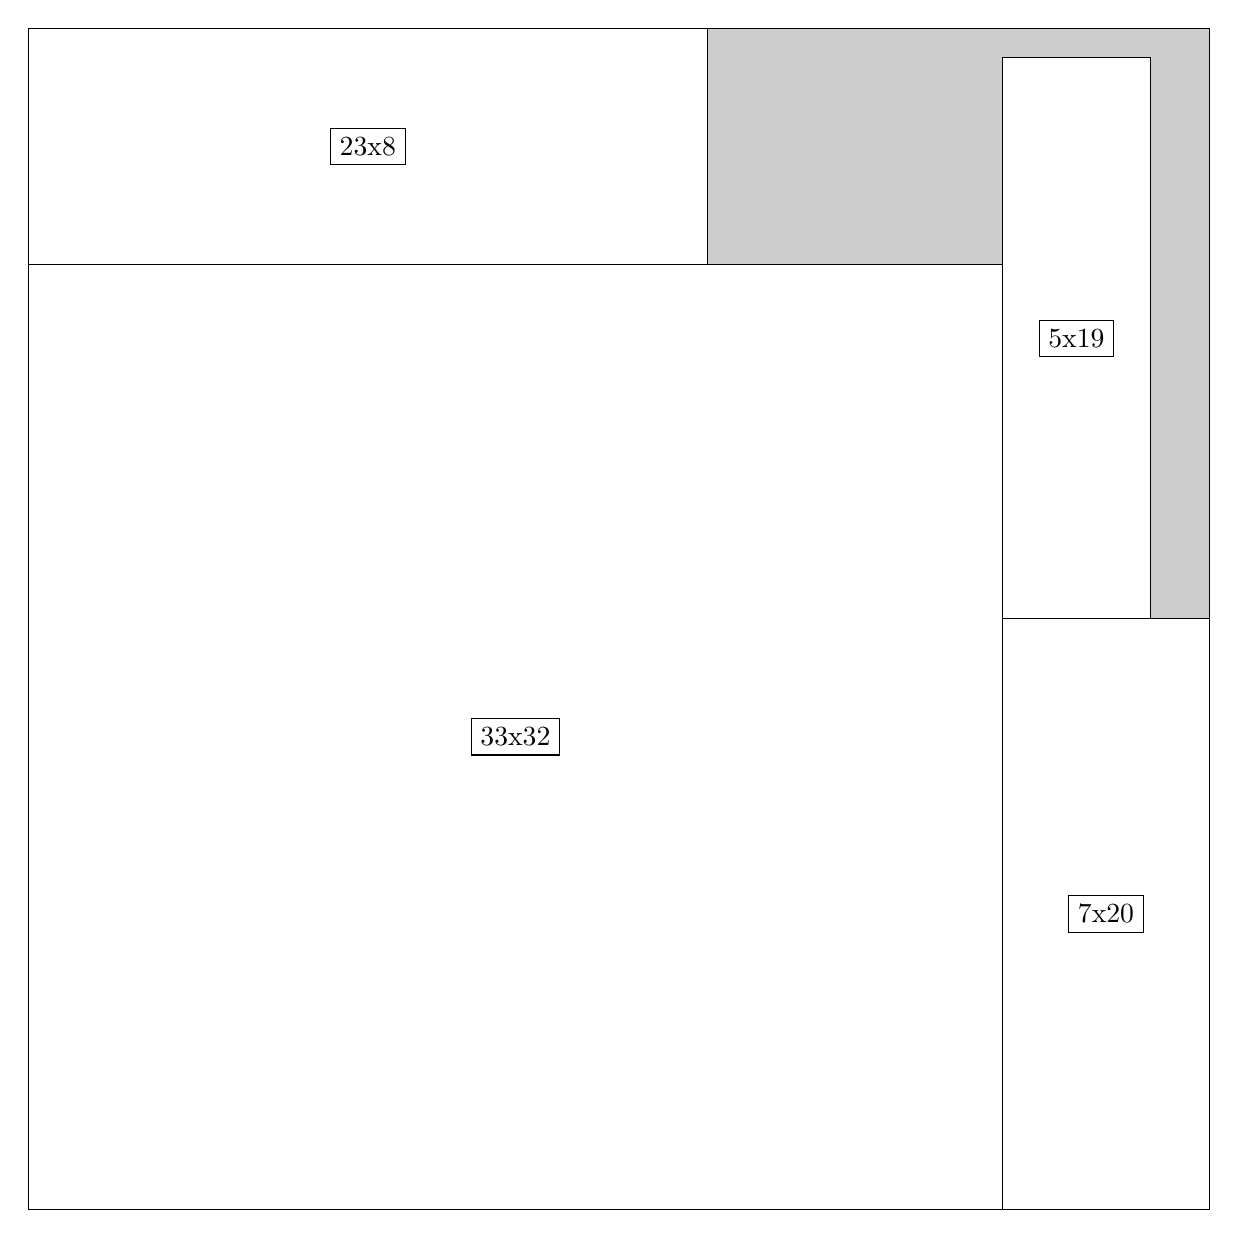
\begin{tikzpicture}[shorten >=1pt,scale=1.0,every node/.style={scale=1.0},->]
\tikzstyle{vertex}=[circle,fill=black!25,minimum size=14pt,inner sep=0pt]
\filldraw[fill=gray!40!white, draw=black] (0,0) rectangle (15.0,15.0);
\foreach \name/\x/\y/\w/\h in {7x20/12.375/0.0/2.625/7.5,33x32/0.0/0.0/12.375/12.0,23x8/0.0/12.0/8.625/3.0,5x19/12.375/7.5/1.875/7.125}
\filldraw[fill=white!40!white, draw=black] (\x,\y) rectangle node[draw] (\name) {\name} ++(\w,\h);
\end{tikzpicture}


w =7 , h =20 , x =33 , y =0 , v =140
\par
w =33 , h =32 , x =0 , y =0 , v =1056
\par
w =23 , h =8 , x =0 , y =32 , v =184
\par
w =5 , h =19 , x =33 , y =20 , v =95
\par
\newpage


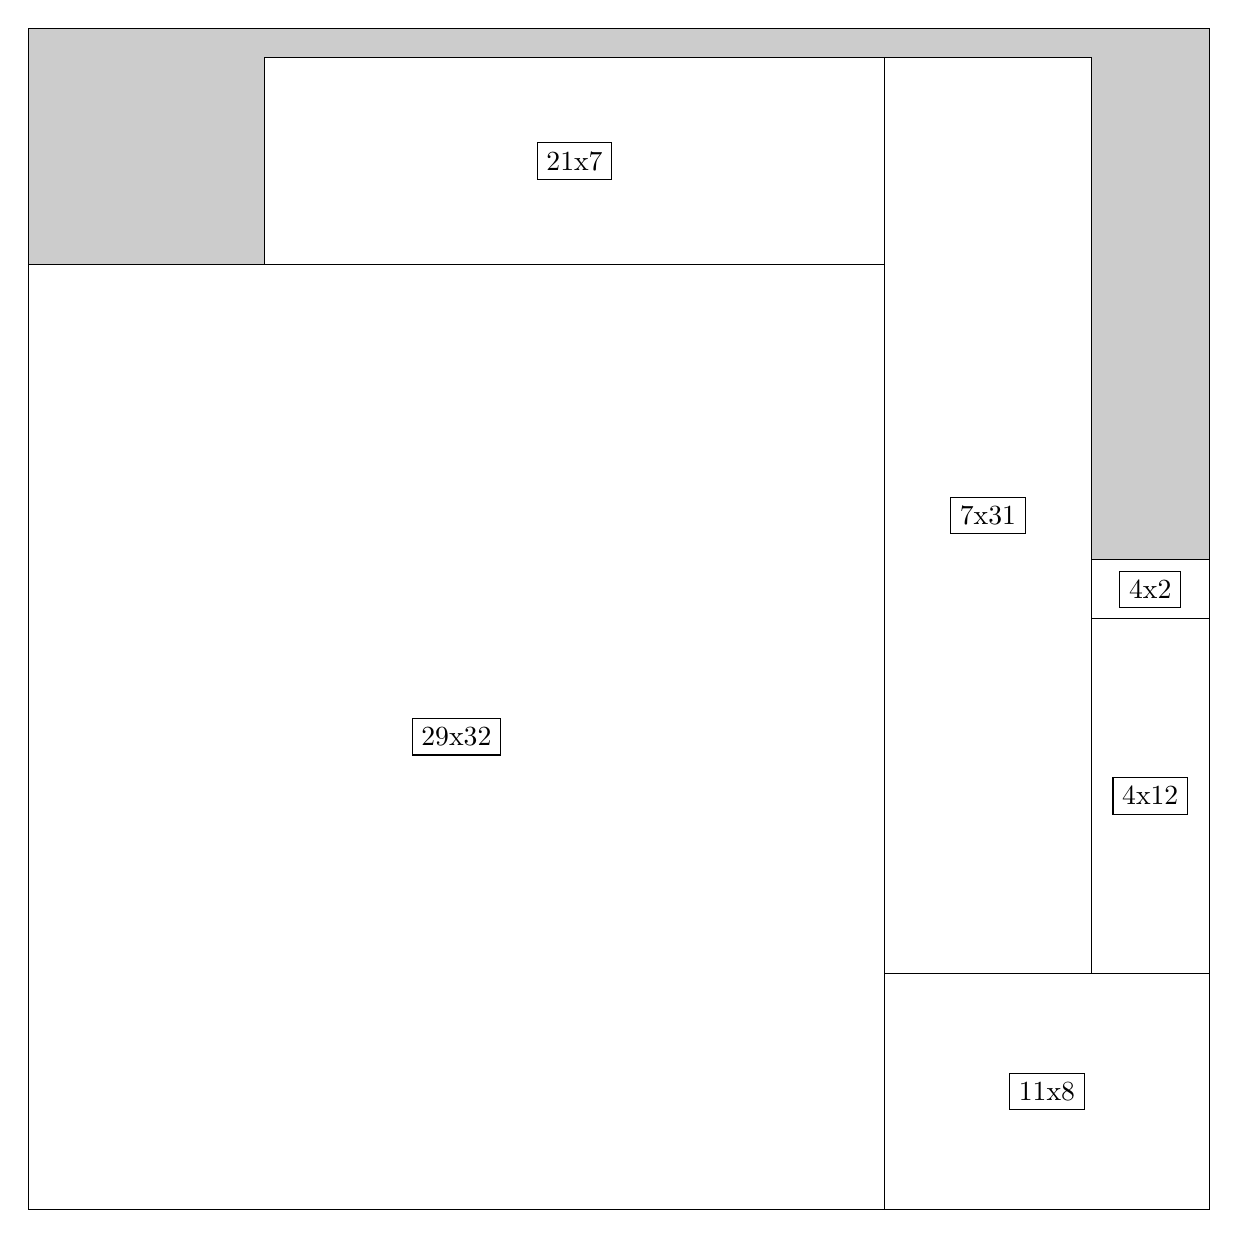
\begin{tikzpicture}[shorten >=1pt,scale=1.0,every node/.style={scale=1.0},->]
\tikzstyle{vertex}=[circle,fill=black!25,minimum size=14pt,inner sep=0pt]
\filldraw[fill=gray!40!white, draw=black] (0,0) rectangle (15.0,15.0);
\foreach \name/\x/\y/\w/\h in {29x32/0.0/0.0/10.875/12.0,11x8/10.875/0.0/4.125/3.0,7x31/10.875/3.0/2.625/11.625,21x7/3.0/12.0/7.875/2.625,4x12/13.5/3.0/1.5/4.5,4x2/13.5/7.5/1.5/0.75}
\filldraw[fill=white!40!white, draw=black] (\x,\y) rectangle node[draw] (\name) {\name} ++(\w,\h);
\end{tikzpicture}


w =29 , h =32 , x =0 , y =0 , v =928
\par
w =11 , h =8 , x =29 , y =0 , v =88
\par
w =7 , h =31 , x =29 , y =8 , v =217
\par
w =21 , h =7 , x =8 , y =32 , v =147
\par
w =4 , h =12 , x =36 , y =8 , v =48
\par
w =4 , h =2 , x =36 , y =20 , v =8
\par
\newpage


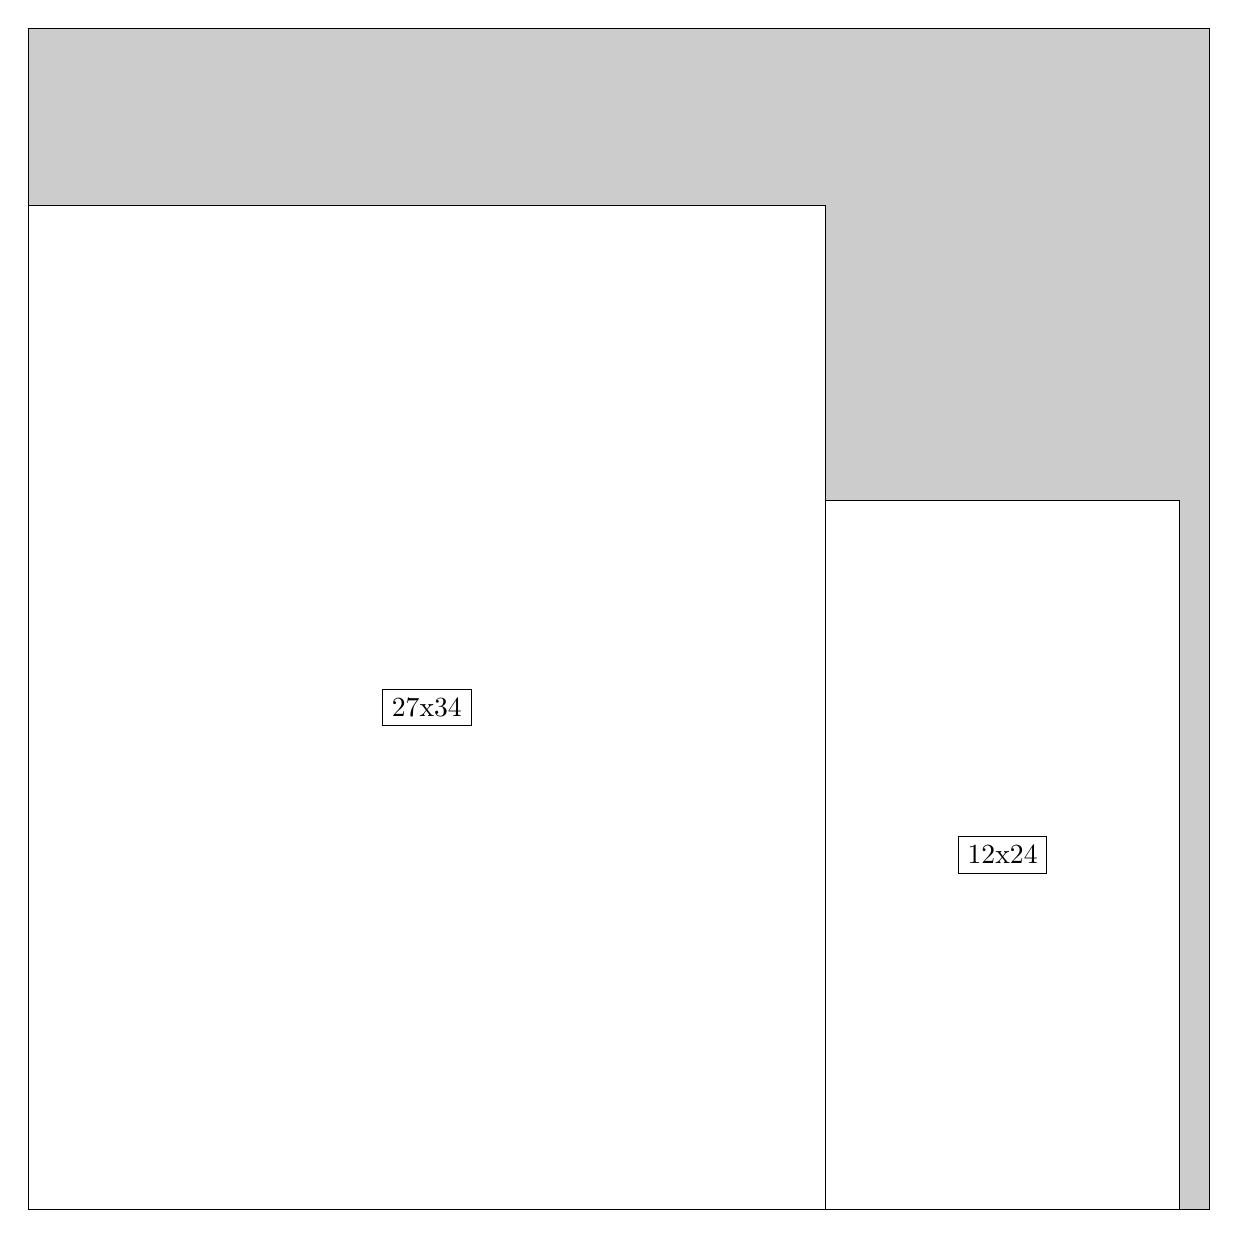
\begin{tikzpicture}[shorten >=1pt,scale=1.0,every node/.style={scale=1.0},->]
\tikzstyle{vertex}=[circle,fill=black!25,minimum size=14pt,inner sep=0pt]
\filldraw[fill=gray!40!white, draw=black] (0,0) rectangle (15.0,15.0);
\foreach \name/\x/\y/\w/\h in {27x34/0.0/0.0/10.125/12.75,12x24/10.125/0.0/4.5/9.0}
\filldraw[fill=white!40!white, draw=black] (\x,\y) rectangle node[draw] (\name) {\name} ++(\w,\h);
\end{tikzpicture}


w =27 , h =34 , x =0 , y =0 , v =918
\par
w =12 , h =24 , x =27 , y =0 , v =288
\par
\newpage


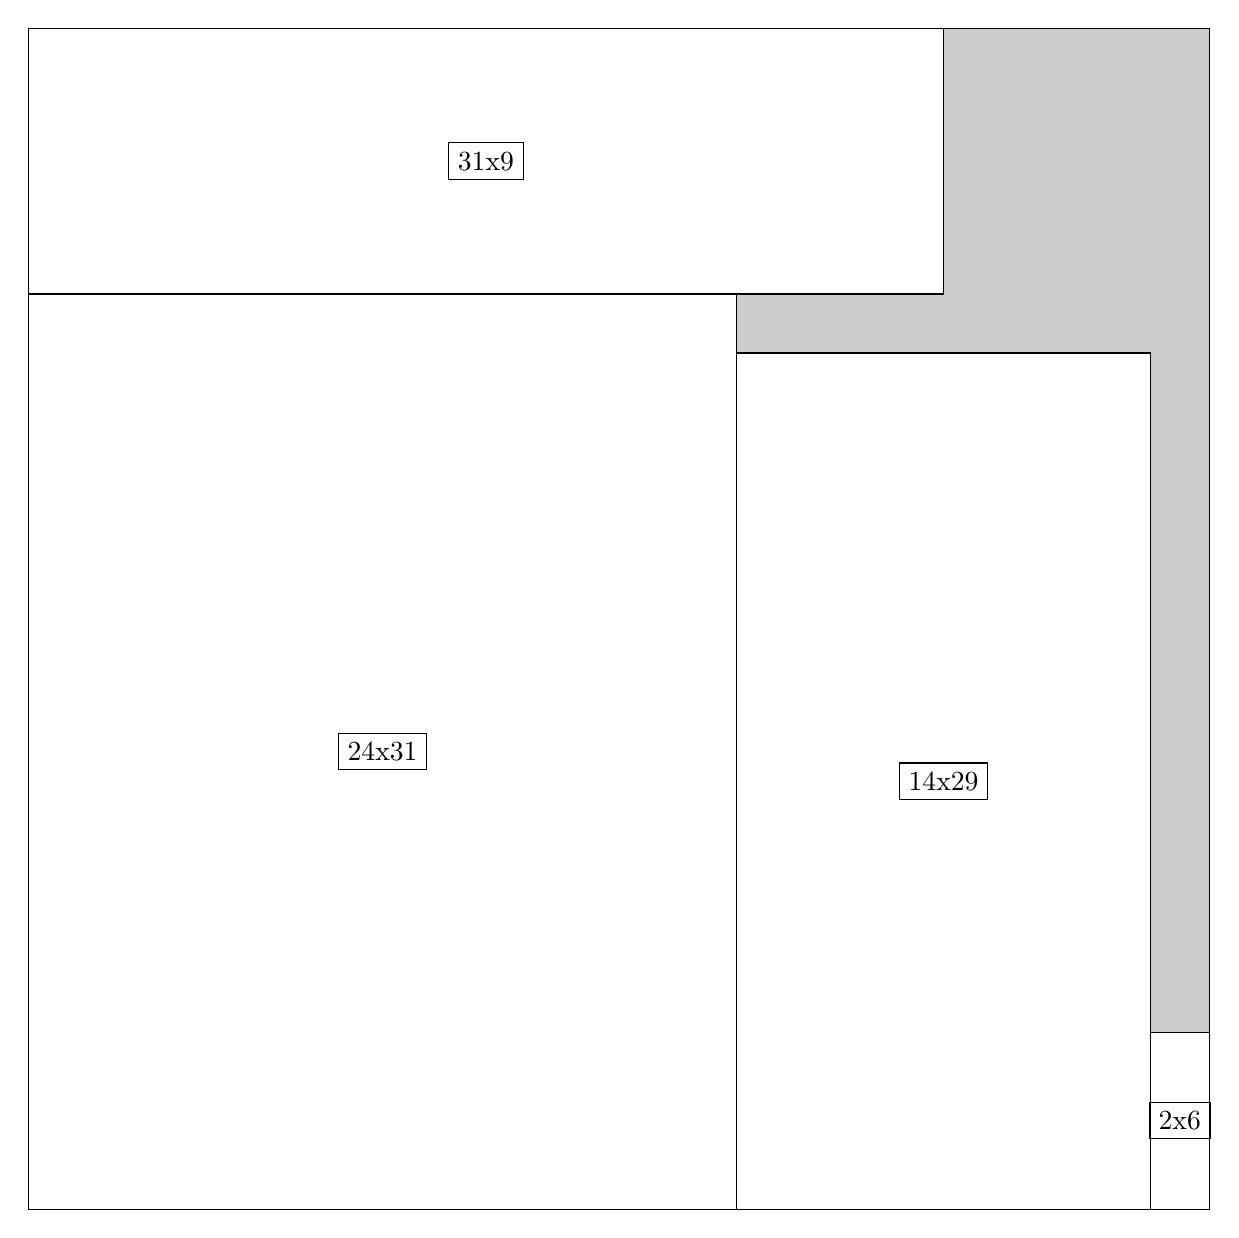
\begin{tikzpicture}[shorten >=1pt,scale=1.0,every node/.style={scale=1.0},->]
\tikzstyle{vertex}=[circle,fill=black!25,minimum size=14pt,inner sep=0pt]
\filldraw[fill=gray!40!white, draw=black] (0,0) rectangle (15.0,15.0);
\foreach \name/\x/\y/\w/\h in {24x31/0.0/0.0/9.0/11.625,14x29/9.0/0.0/5.25/10.875,31x9/0.0/11.625/11.625/3.375,2x6/14.25/0.0/0.75/2.25}
\filldraw[fill=white!40!white, draw=black] (\x,\y) rectangle node[draw] (\name) {\name} ++(\w,\h);
\end{tikzpicture}


w =24 , h =31 , x =0 , y =0 , v =744
\par
w =14 , h =29 , x =24 , y =0 , v =406
\par
w =31 , h =9 , x =0 , y =31 , v =279
\par
w =2 , h =6 , x =38 , y =0 , v =12
\par
\newpage


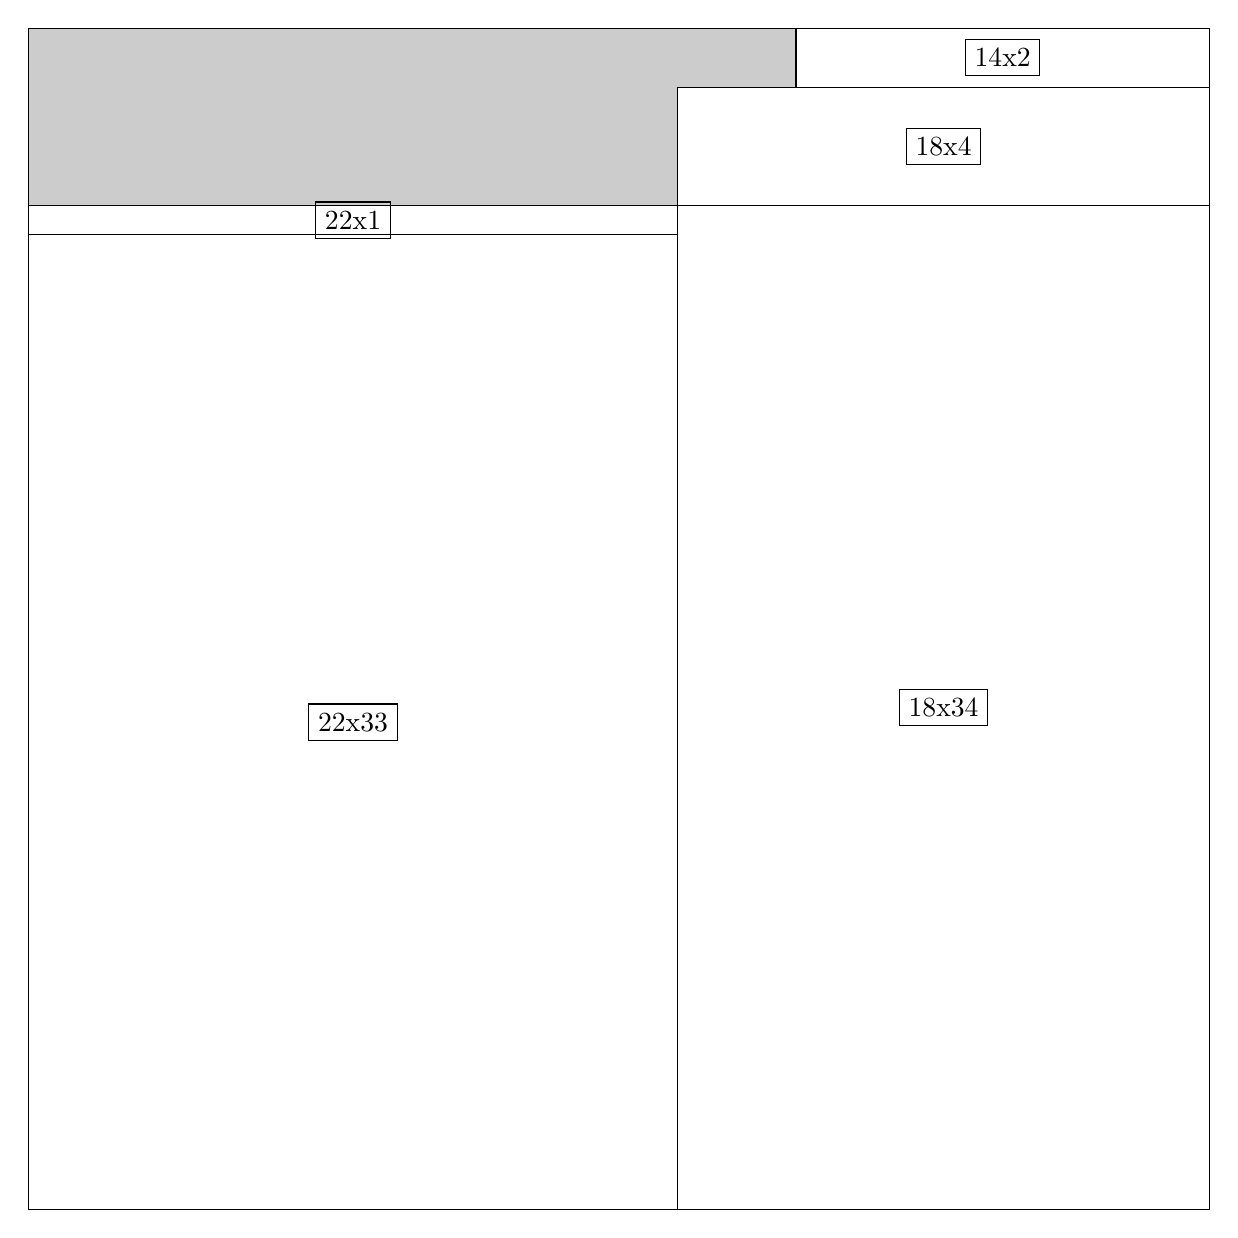
\begin{tikzpicture}[shorten >=1pt,scale=1.0,every node/.style={scale=1.0},->]
\tikzstyle{vertex}=[circle,fill=black!25,minimum size=14pt,inner sep=0pt]
\filldraw[fill=gray!40!white, draw=black] (0,0) rectangle (15.0,15.0);
\foreach \name/\x/\y/\w/\h in {22x33/0.0/0.0/8.25/12.375,18x34/8.25/0.0/6.75/12.75,18x4/8.25/12.75/6.75/1.5,14x2/9.75/14.25/5.25/0.75,22x1/0.0/12.375/8.25/0.375}
\filldraw[fill=white!40!white, draw=black] (\x,\y) rectangle node[draw] (\name) {\name} ++(\w,\h);
\end{tikzpicture}


w =22 , h =33 , x =0 , y =0 , v =726
\par
w =18 , h =34 , x =22 , y =0 , v =612
\par
w =18 , h =4 , x =22 , y =34 , v =72
\par
w =14 , h =2 , x =26 , y =38 , v =28
\par
w =22 , h =1 , x =0 , y =33 , v =22
\par
\newpage


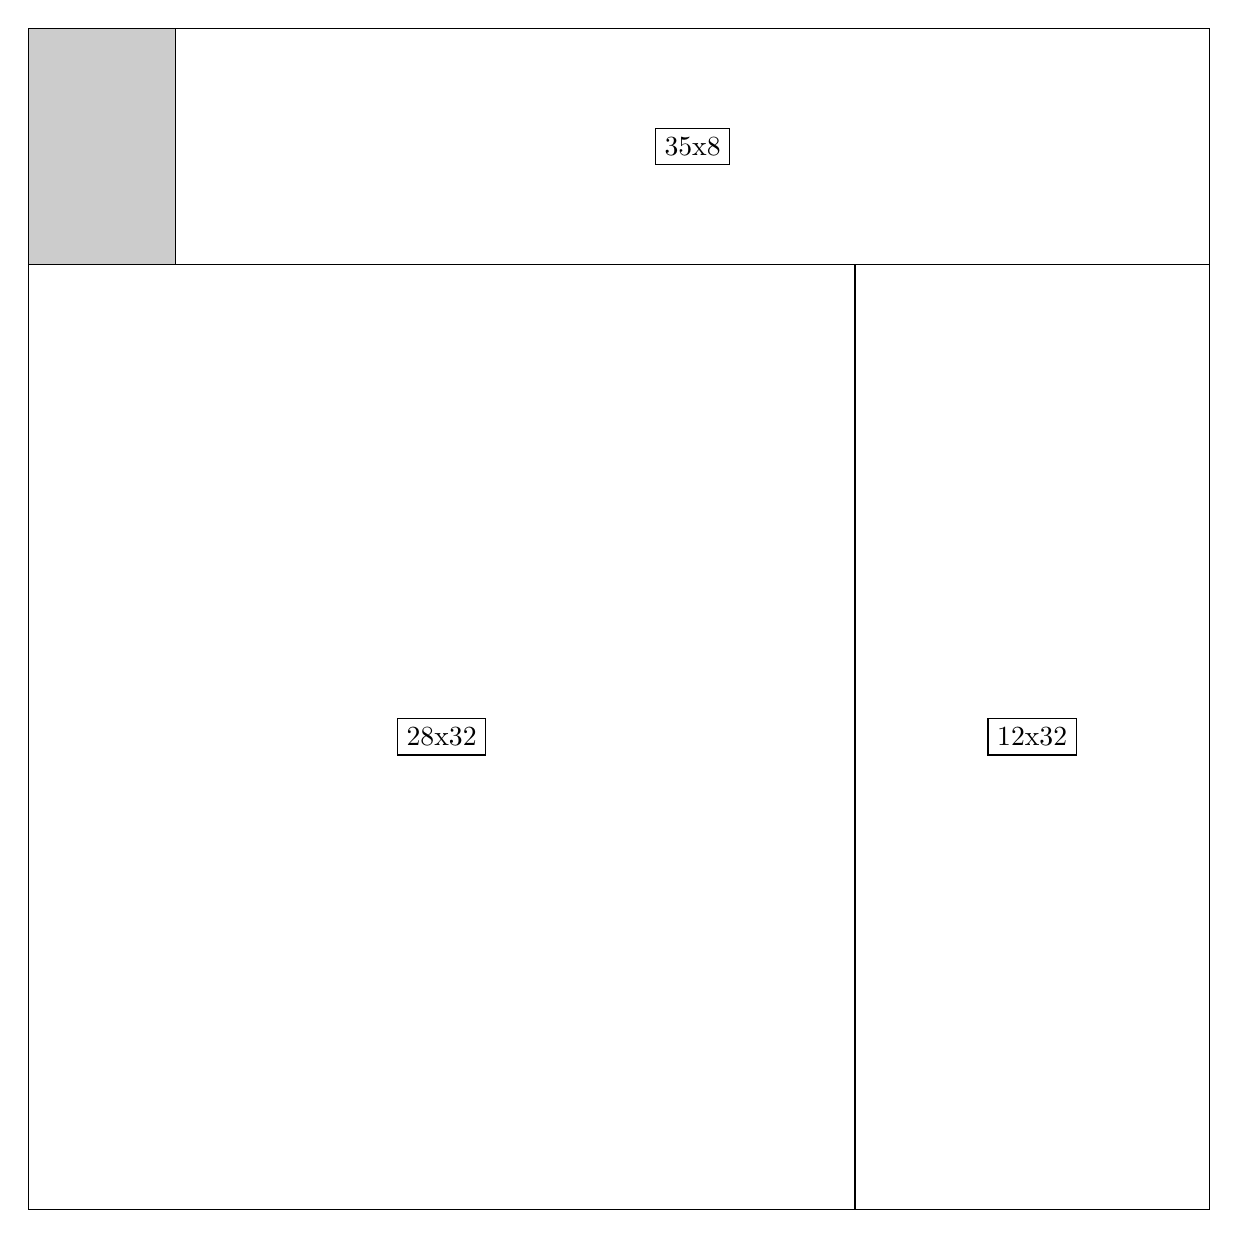
\begin{tikzpicture}[shorten >=1pt,scale=1.0,every node/.style={scale=1.0},->]
\tikzstyle{vertex}=[circle,fill=black!25,minimum size=14pt,inner sep=0pt]
\filldraw[fill=gray!40!white, draw=black] (0,0) rectangle (15.0,15.0);
\foreach \name/\x/\y/\w/\h in {12x32/10.5/0.0/4.5/12.0,28x32/0.0/0.0/10.5/12.0,35x8/1.875/12.0/13.125/3.0}
\filldraw[fill=white!40!white, draw=black] (\x,\y) rectangle node[draw] (\name) {\name} ++(\w,\h);
\end{tikzpicture}


w =12 , h =32 , x =28 , y =0 , v =384
\par
w =28 , h =32 , x =0 , y =0 , v =896
\par
w =35 , h =8 , x =5 , y =32 , v =280
\par
\newpage


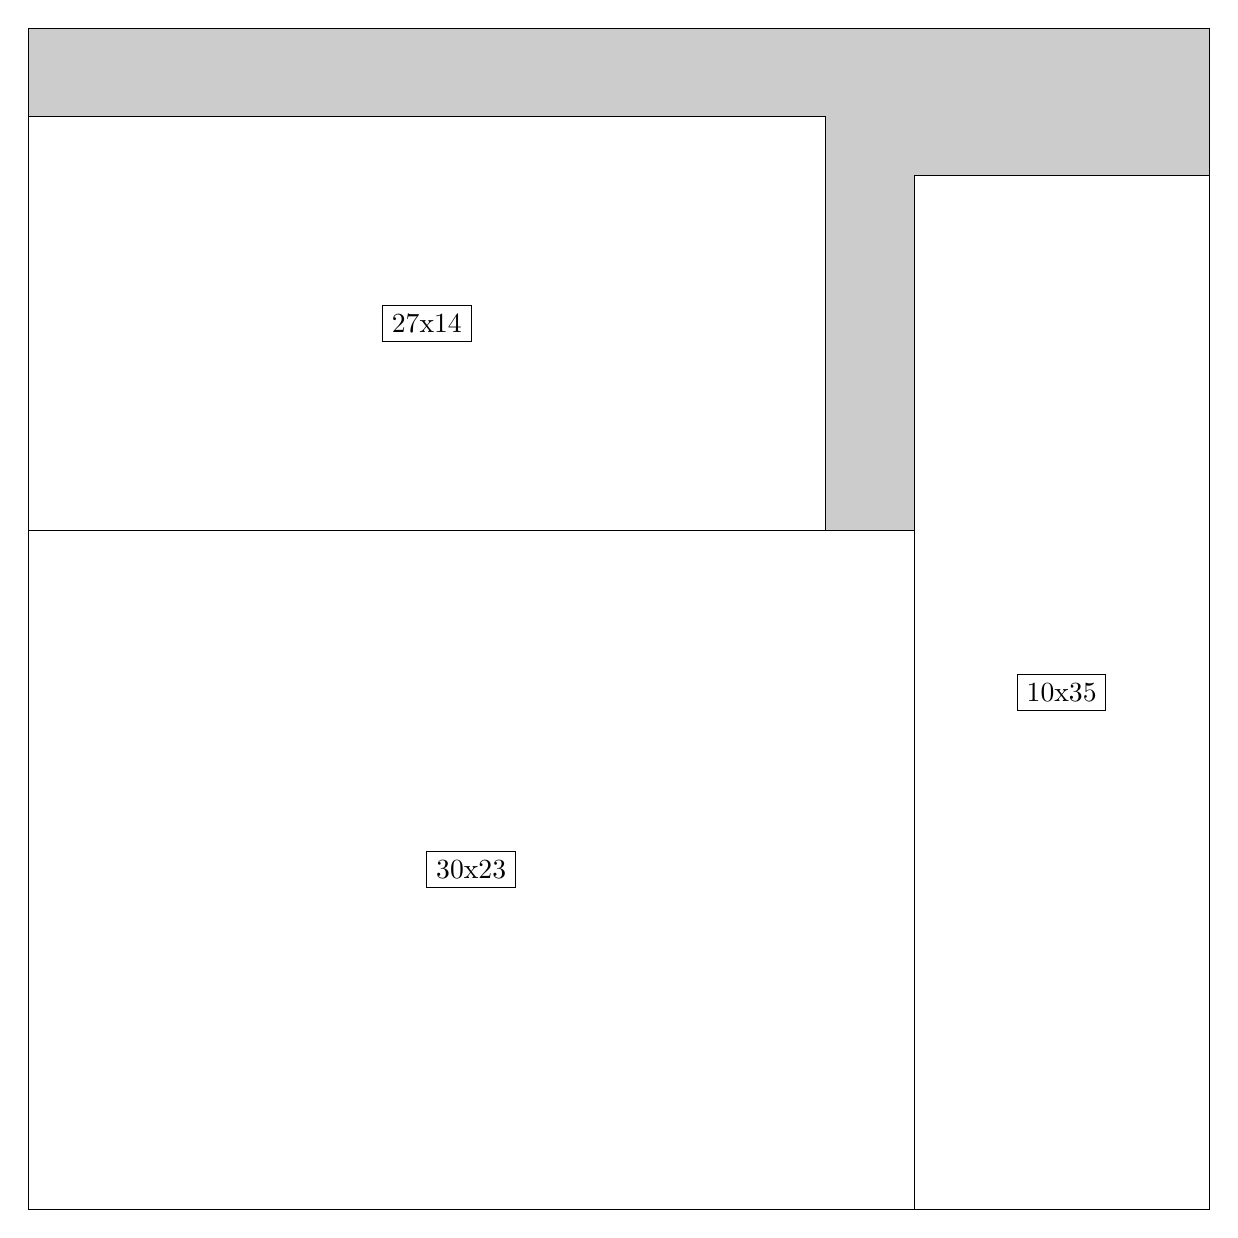
\begin{tikzpicture}[shorten >=1pt,scale=1.0,every node/.style={scale=1.0},->]
\tikzstyle{vertex}=[circle,fill=black!25,minimum size=14pt,inner sep=0pt]
\filldraw[fill=gray!40!white, draw=black] (0,0) rectangle (15.0,15.0);
\foreach \name/\x/\y/\w/\h in {30x23/0.0/0.0/11.25/8.625,27x14/0.0/8.625/10.125/5.25,10x35/11.25/0.0/3.75/13.125}
\filldraw[fill=white!40!white, draw=black] (\x,\y) rectangle node[draw] (\name) {\name} ++(\w,\h);
\end{tikzpicture}


w =30 , h =23 , x =0 , y =0 , v =690
\par
w =27 , h =14 , x =0 , y =23 , v =378
\par
w =10 , h =35 , x =30 , y =0 , v =350
\par
\newpage


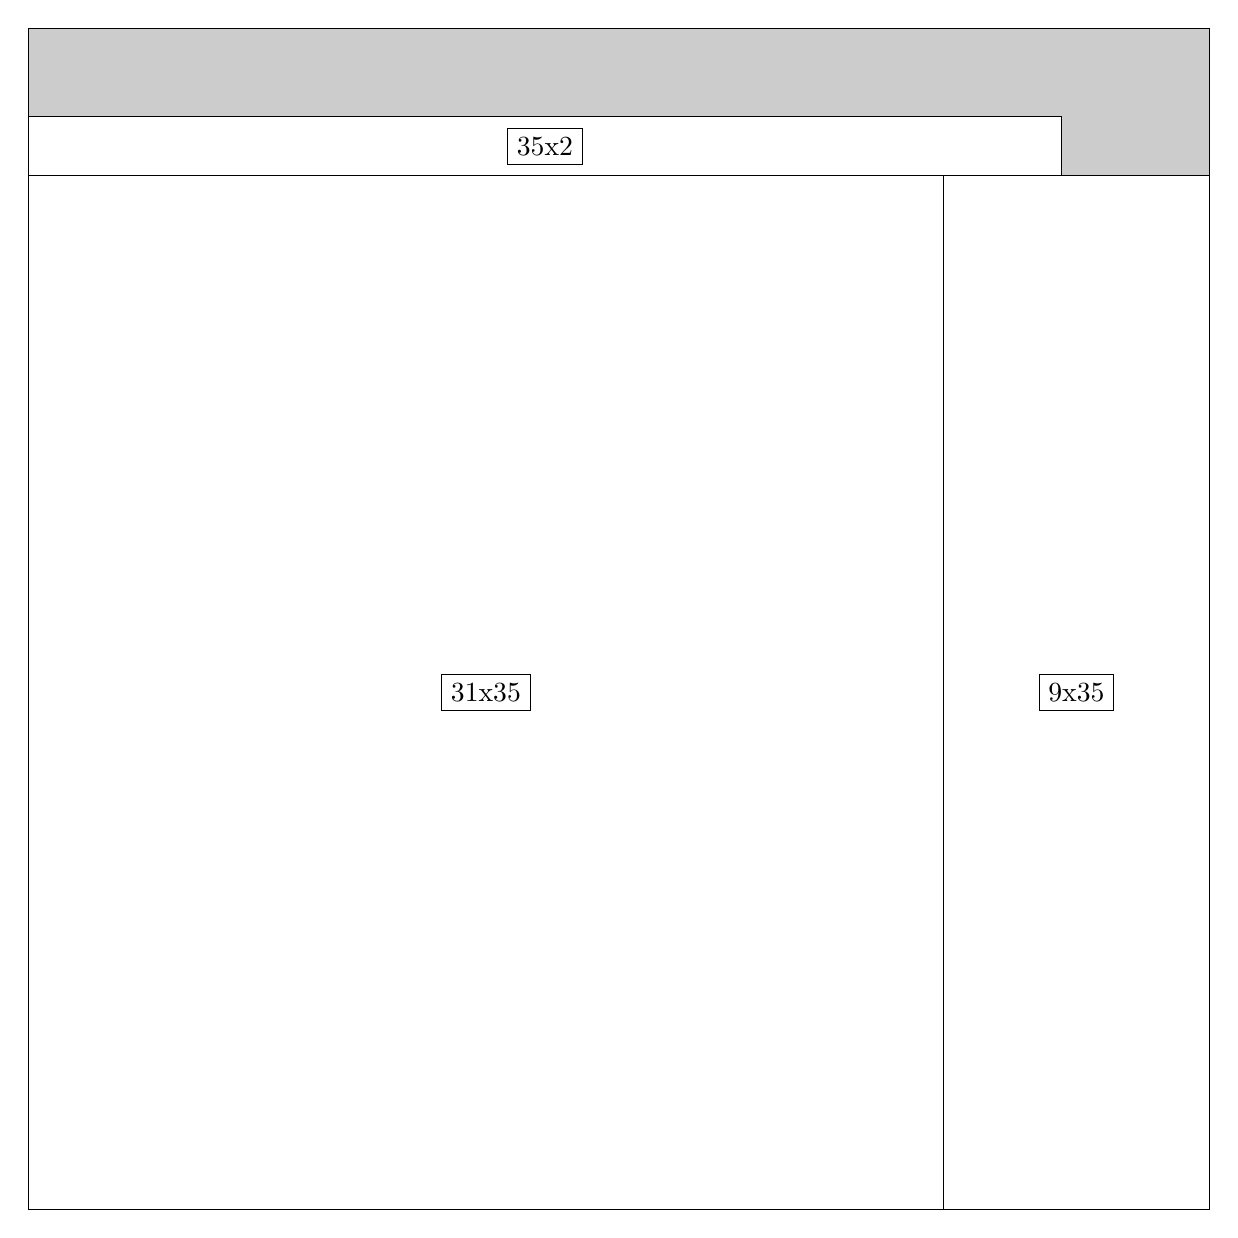
\begin{tikzpicture}[shorten >=1pt,scale=1.0,every node/.style={scale=1.0},->]
\tikzstyle{vertex}=[circle,fill=black!25,minimum size=14pt,inner sep=0pt]
\filldraw[fill=gray!40!white, draw=black] (0,0) rectangle (15.0,15.0);
\foreach \name/\x/\y/\w/\h in {31x35/0.0/0.0/11.625/13.125,9x35/11.625/0.0/3.375/13.125,35x2/0.0/13.125/13.125/0.75}
\filldraw[fill=white!40!white, draw=black] (\x,\y) rectangle node[draw] (\name) {\name} ++(\w,\h);
\end{tikzpicture}


w =31 , h =35 , x =0 , y =0 , v =1085
\par
w =9 , h =35 , x =31 , y =0 , v =315
\par
w =35 , h =2 , x =0 , y =35 , v =70
\par
\newpage


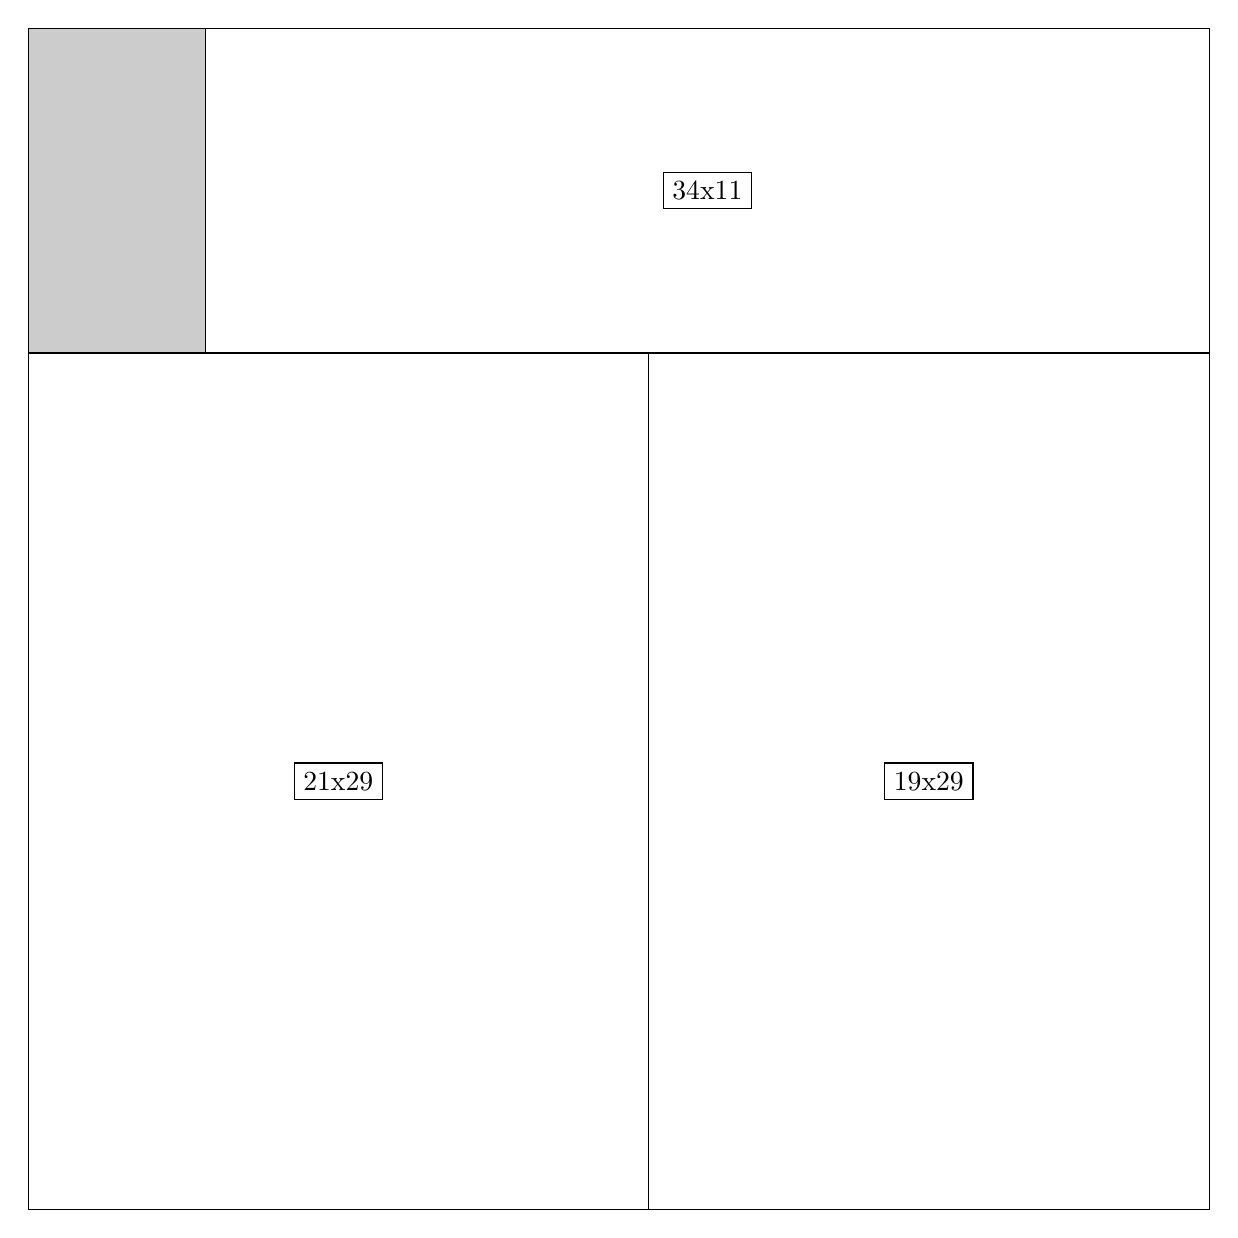
\begin{tikzpicture}[shorten >=1pt,scale=1.0,every node/.style={scale=1.0},->]
\tikzstyle{vertex}=[circle,fill=black!25,minimum size=14pt,inner sep=0pt]
\filldraw[fill=gray!40!white, draw=black] (0,0) rectangle (15.0,15.0);
\foreach \name/\x/\y/\w/\h in {19x29/7.875/0.0/7.125/10.875,21x29/0.0/0.0/7.875/10.875,34x11/2.25/10.875/12.75/4.125}
\filldraw[fill=white!40!white, draw=black] (\x,\y) rectangle node[draw] (\name) {\name} ++(\w,\h);
\end{tikzpicture}


w =19 , h =29 , x =21 , y =0 , v =551
\par
w =21 , h =29 , x =0 , y =0 , v =609
\par
w =34 , h =11 , x =6 , y =29 , v =374
\par
\newpage


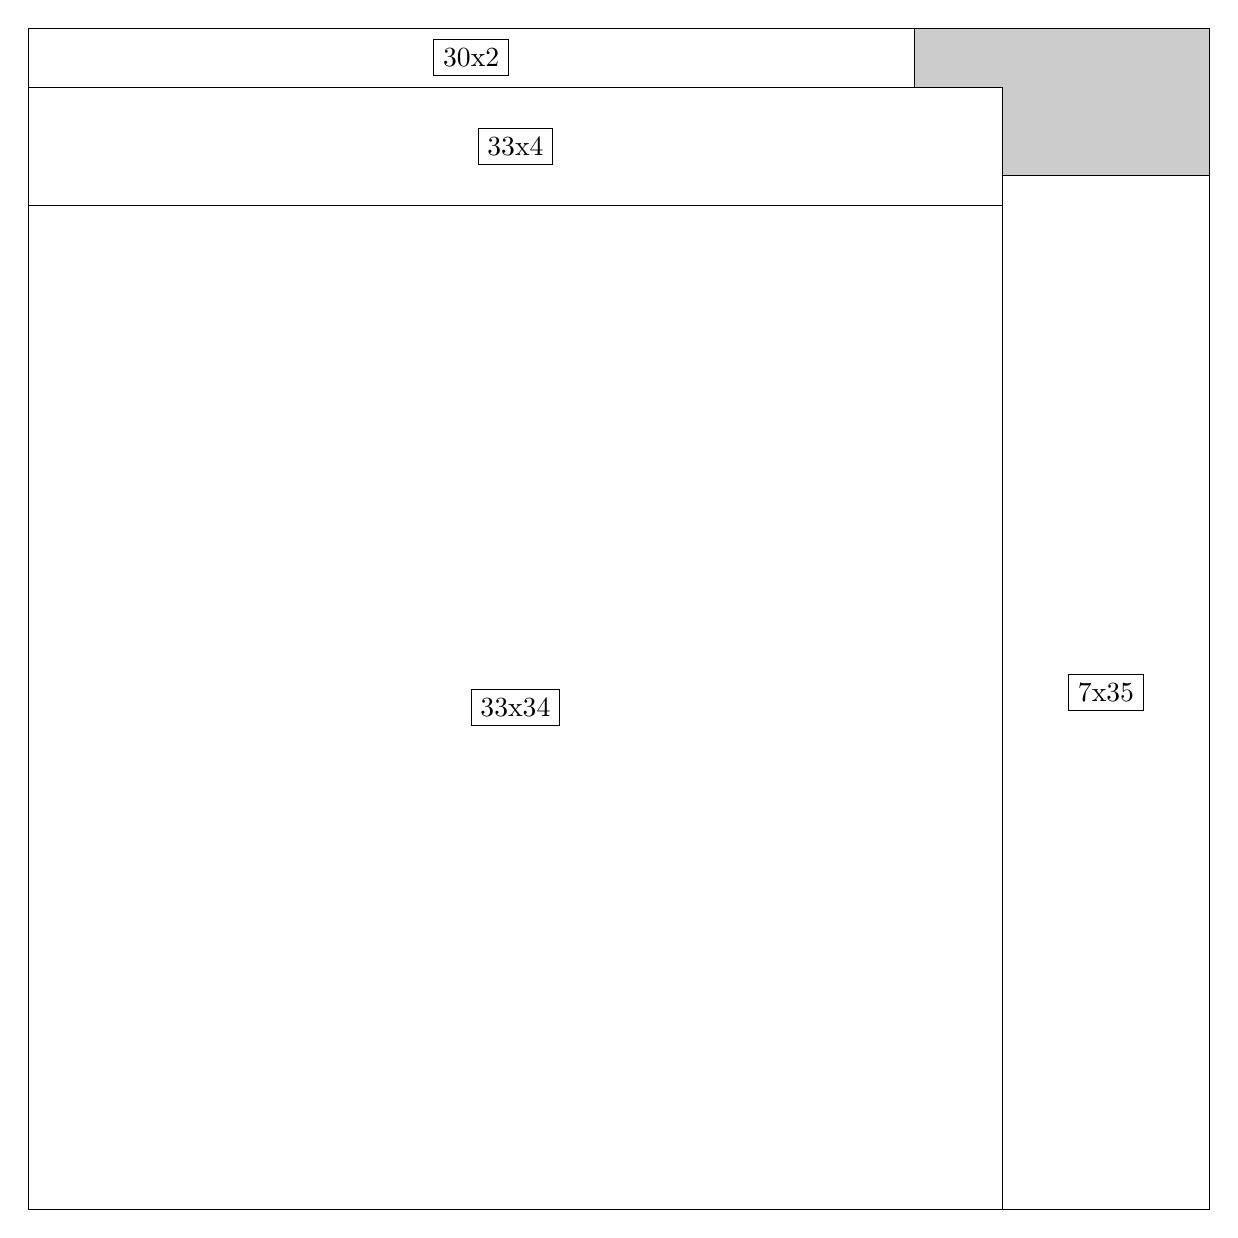
\begin{tikzpicture}[shorten >=1pt,scale=1.0,every node/.style={scale=1.0},->]
\tikzstyle{vertex}=[circle,fill=black!25,minimum size=14pt,inner sep=0pt]
\filldraw[fill=gray!40!white, draw=black] (0,0) rectangle (15.0,15.0);
\foreach \name/\x/\y/\w/\h in {33x34/0.0/0.0/12.375/12.75,7x35/12.375/0.0/2.625/13.125,33x4/0.0/12.75/12.375/1.5,30x2/0.0/14.25/11.25/0.75}
\filldraw[fill=white!40!white, draw=black] (\x,\y) rectangle node[draw] (\name) {\name} ++(\w,\h);
\end{tikzpicture}


w =33 , h =34 , x =0 , y =0 , v =1122
\par
w =7 , h =35 , x =33 , y =0 , v =245
\par
w =33 , h =4 , x =0 , y =34 , v =132
\par
w =30 , h =2 , x =0 , y =38 , v =60
\par
\newpage


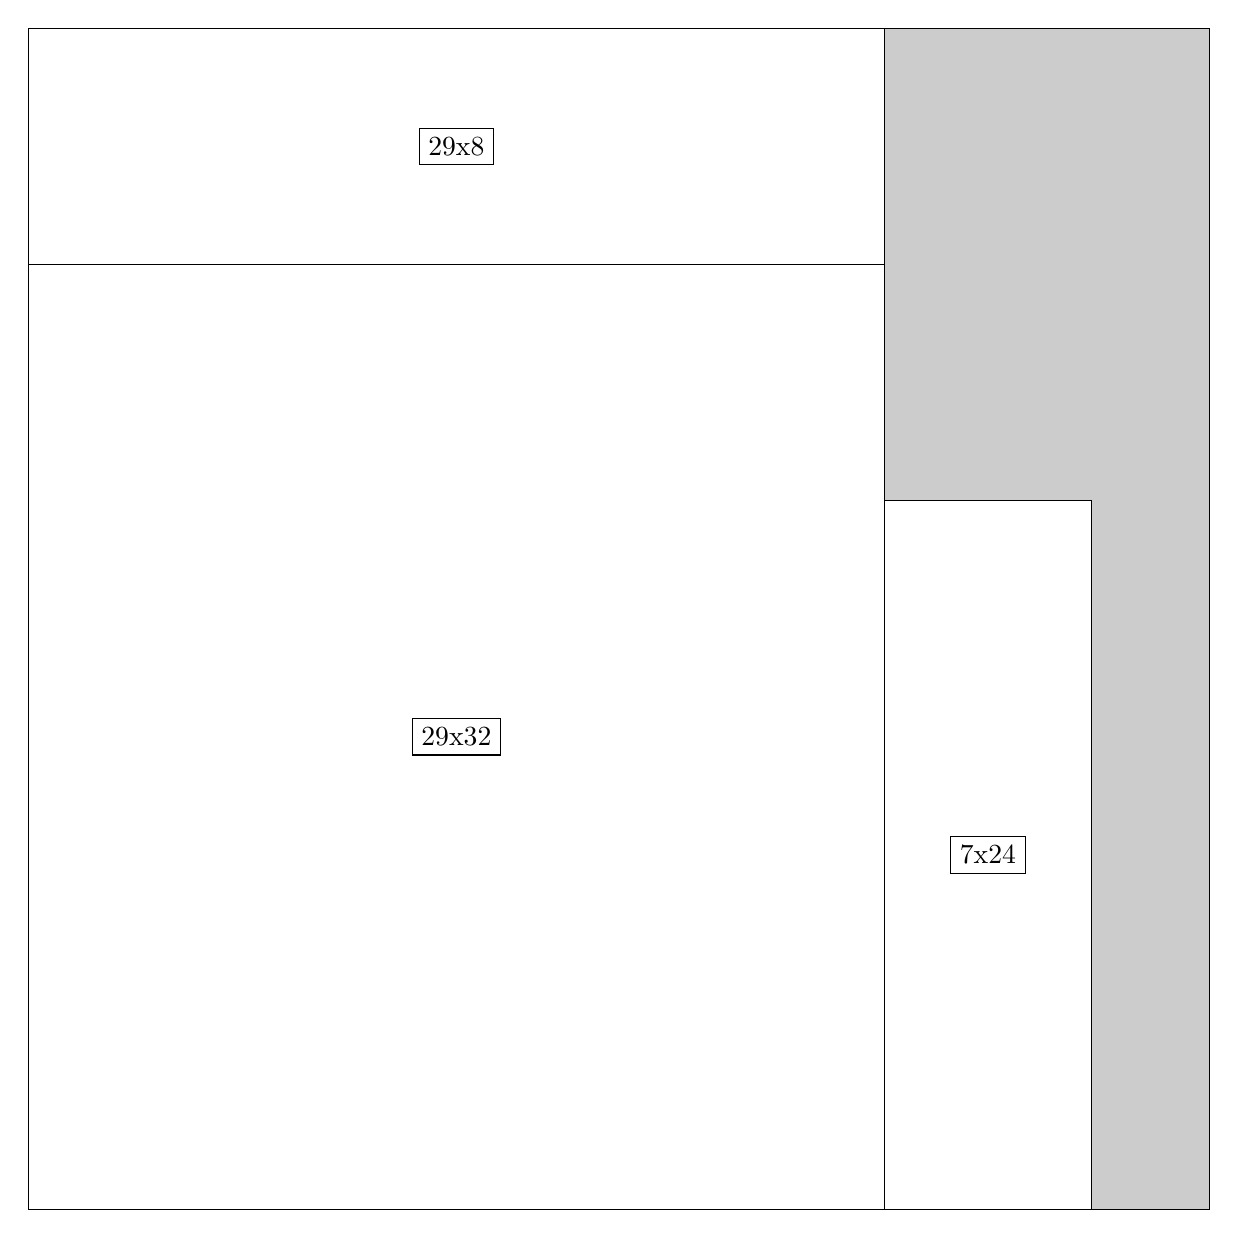
\begin{tikzpicture}[shorten >=1pt,scale=1.0,every node/.style={scale=1.0},->]
\tikzstyle{vertex}=[circle,fill=black!25,minimum size=14pt,inner sep=0pt]
\filldraw[fill=gray!40!white, draw=black] (0,0) rectangle (15.0,15.0);
\foreach \name/\x/\y/\w/\h in {29x32/0.0/0.0/10.875/12.0,7x24/10.875/0.0/2.625/9.0,29x8/0.0/12.0/10.875/3.0}
\filldraw[fill=white!40!white, draw=black] (\x,\y) rectangle node[draw] (\name) {\name} ++(\w,\h);
\end{tikzpicture}


w =29 , h =32 , x =0 , y =0 , v =928
\par
w =7 , h =24 , x =29 , y =0 , v =168
\par
w =29 , h =8 , x =0 , y =32 , v =232
\par
\newpage


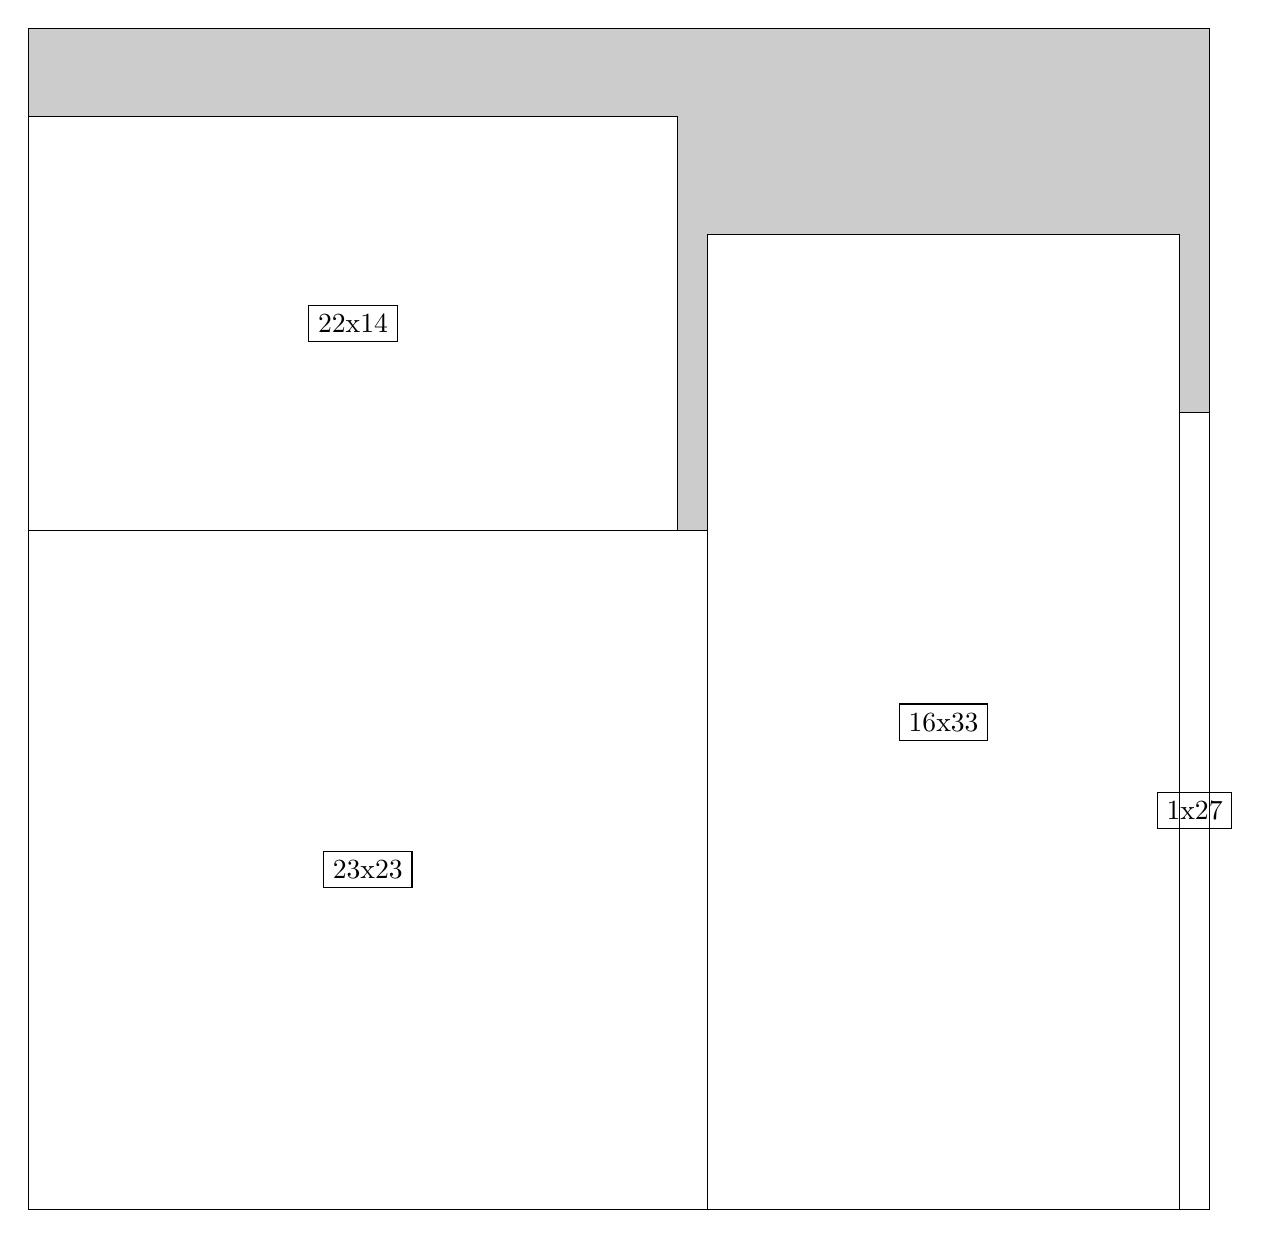
\begin{tikzpicture}[shorten >=1pt,scale=1.0,every node/.style={scale=1.0},->]
\tikzstyle{vertex}=[circle,fill=black!25,minimum size=14pt,inner sep=0pt]
\filldraw[fill=gray!40!white, draw=black] (0,0) rectangle (15.0,15.0);
\foreach \name/\x/\y/\w/\h in {23x23/0.0/0.0/8.625/8.625,16x33/8.625/0.0/6.0/12.375,22x14/0.0/8.625/8.25/5.25,1x27/14.625/0.0/0.375/10.125}
\filldraw[fill=white!40!white, draw=black] (\x,\y) rectangle node[draw] (\name) {\name} ++(\w,\h);
\end{tikzpicture}


w =23 , h =23 , x =0 , y =0 , v =529
\par
w =16 , h =33 , x =23 , y =0 , v =528
\par
w =22 , h =14 , x =0 , y =23 , v =308
\par
w =1 , h =27 , x =39 , y =0 , v =27
\par
\newpage


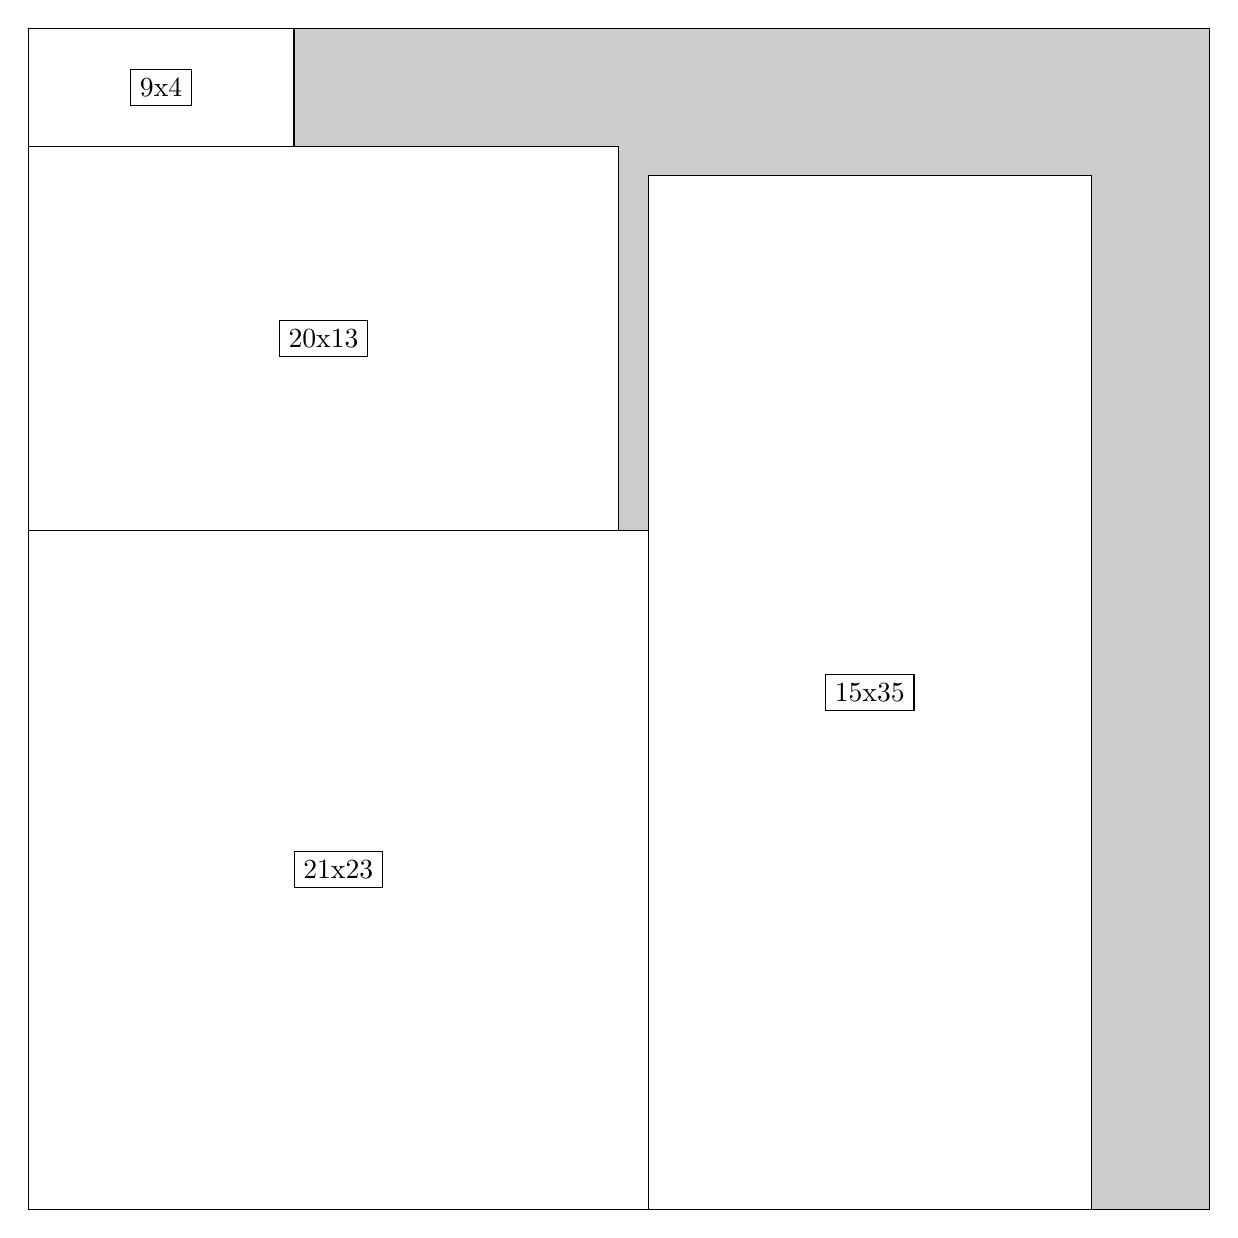
\begin{tikzpicture}[shorten >=1pt,scale=1.0,every node/.style={scale=1.0},->]
\tikzstyle{vertex}=[circle,fill=black!25,minimum size=14pt,inner sep=0pt]
\filldraw[fill=gray!40!white, draw=black] (0,0) rectangle (15.0,15.0);
\foreach \name/\x/\y/\w/\h in {15x35/7.875/0.0/5.625/13.125,21x23/0.0/0.0/7.875/8.625,20x13/0.0/8.625/7.5/4.875,9x4/0.0/13.5/3.375/1.5}
\filldraw[fill=white!40!white, draw=black] (\x,\y) rectangle node[draw] (\name) {\name} ++(\w,\h);
\end{tikzpicture}


w =15 , h =35 , x =21 , y =0 , v =525
\par
w =21 , h =23 , x =0 , y =0 , v =483
\par
w =20 , h =13 , x =0 , y =23 , v =260
\par
w =9 , h =4 , x =0 , y =36 , v =36
\par
\newpage


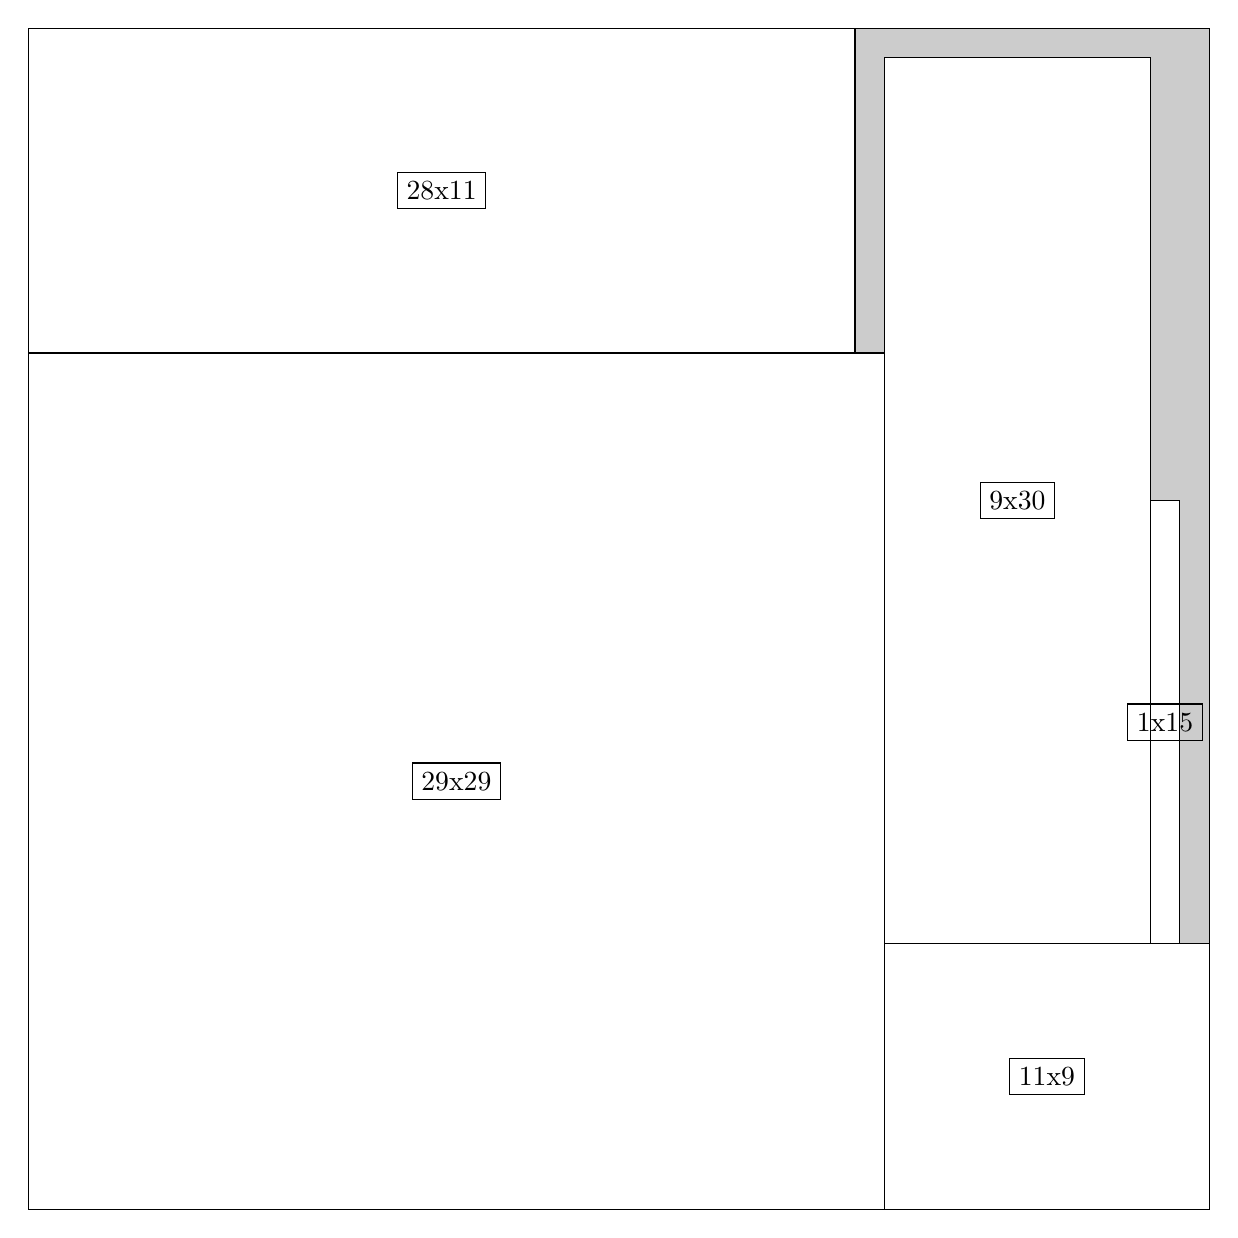
\begin{tikzpicture}[shorten >=1pt,scale=1.0,every node/.style={scale=1.0},->]
\tikzstyle{vertex}=[circle,fill=black!25,minimum size=14pt,inner sep=0pt]
\filldraw[fill=gray!40!white, draw=black] (0,0) rectangle (15.0,15.0);
\foreach \name/\x/\y/\w/\h in {29x29/0.0/0.0/10.875/10.875,28x11/0.0/10.875/10.5/4.125,11x9/10.875/0.0/4.125/3.375,9x30/10.875/3.375/3.375/11.25,1x15/14.25/3.375/0.375/5.625}
\filldraw[fill=white!40!white, draw=black] (\x,\y) rectangle node[draw] (\name) {\name} ++(\w,\h);
\end{tikzpicture}


w =29 , h =29 , x =0 , y =0 , v =841
\par
w =28 , h =11 , x =0 , y =29 , v =308
\par
w =11 , h =9 , x =29 , y =0 , v =99
\par
w =9 , h =30 , x =29 , y =9 , v =270
\par
w =1 , h =15 , x =38 , y =9 , v =15
\par
\newpage


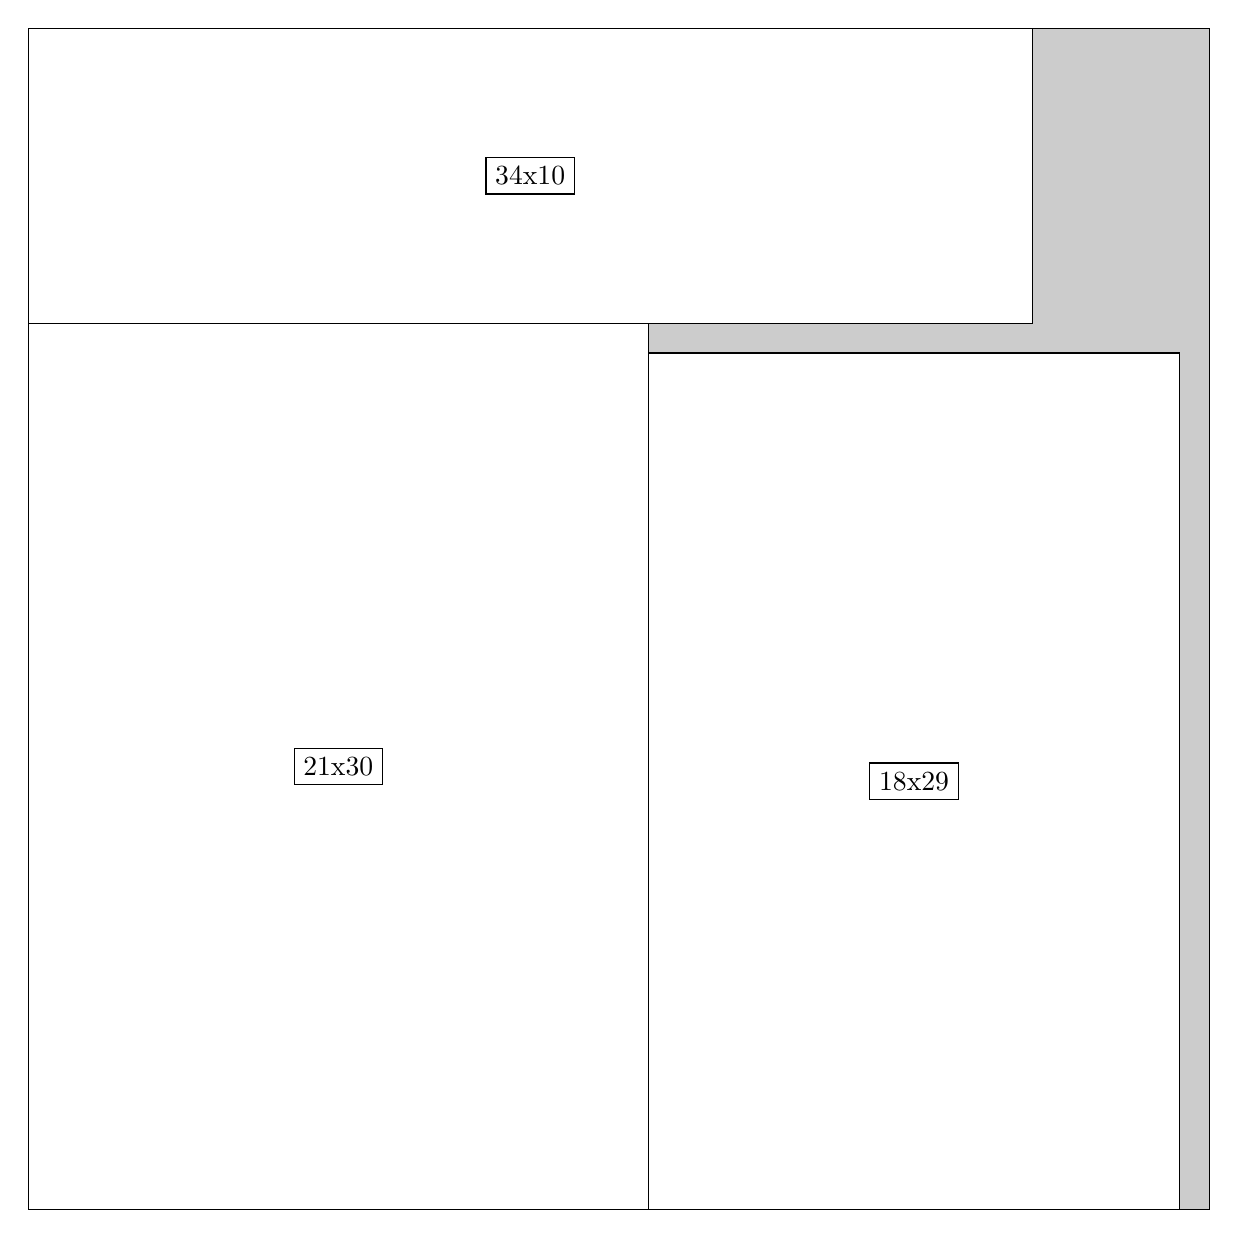
\begin{tikzpicture}[shorten >=1pt,scale=1.0,every node/.style={scale=1.0},->]
\tikzstyle{vertex}=[circle,fill=black!25,minimum size=14pt,inner sep=0pt]
\filldraw[fill=gray!40!white, draw=black] (0,0) rectangle (15.0,15.0);
\foreach \name/\x/\y/\w/\h in {18x29/7.875/0.0/6.75/10.875,34x10/0.0/11.25/12.75/3.75,21x30/0.0/0.0/7.875/11.25}
\filldraw[fill=white!40!white, draw=black] (\x,\y) rectangle node[draw] (\name) {\name} ++(\w,\h);
\end{tikzpicture}


w =18 , h =29 , x =21 , y =0 , v =522
\par
w =34 , h =10 , x =0 , y =30 , v =340
\par
w =21 , h =30 , x =0 , y =0 , v =630
\par
\newpage


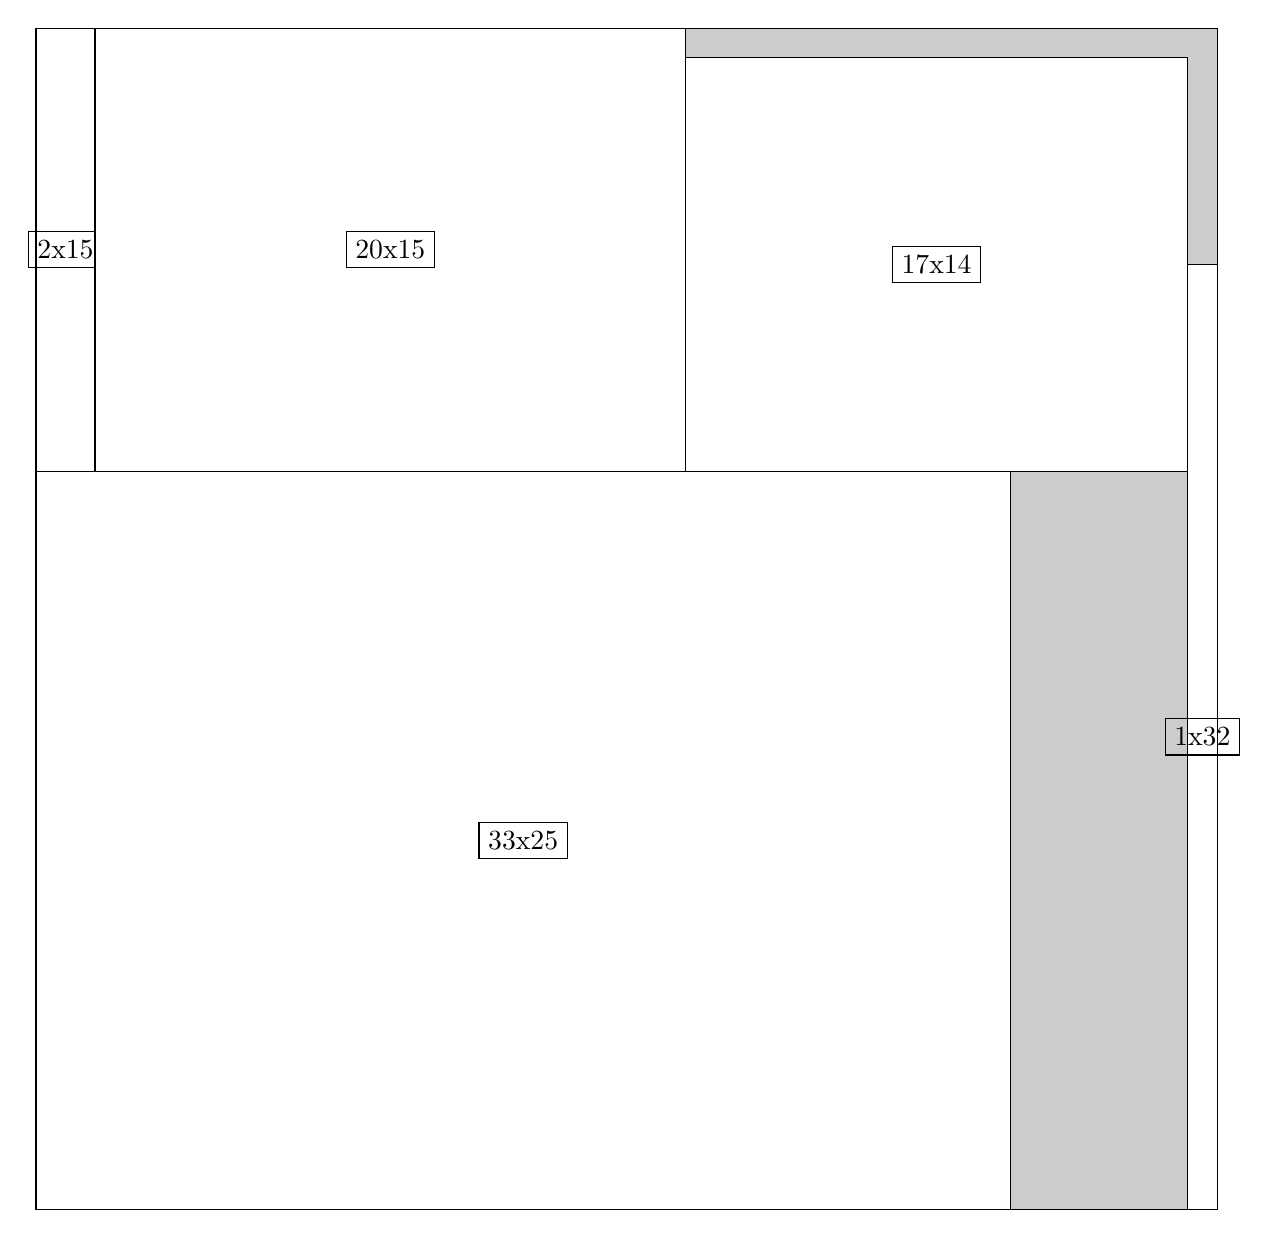
\begin{tikzpicture}[shorten >=1pt,scale=1.0,every node/.style={scale=1.0},->]
\tikzstyle{vertex}=[circle,fill=black!25,minimum size=14pt,inner sep=0pt]
\filldraw[fill=gray!40!white, draw=black] (0,0) rectangle (15.0,15.0);
\foreach \name/\x/\y/\w/\h in {2x15/0.0/9.375/0.75/5.625,20x15/0.75/9.375/7.5/5.625,17x14/8.25/9.375/6.375/5.25,33x25/0.0/0.0/12.375/9.375,1x32/14.625/0.0/0.375/12.0}
\filldraw[fill=white!40!white, draw=black] (\x,\y) rectangle node[draw] (\name) {\name} ++(\w,\h);
\end{tikzpicture}


w =2 , h =15 , x =0 , y =25 , v =30
\par
w =20 , h =15 , x =2 , y =25 , v =300
\par
w =17 , h =14 , x =22 , y =25 , v =238
\par
w =33 , h =25 , x =0 , y =0 , v =825
\par
w =1 , h =32 , x =39 , y =0 , v =32
\par
\newpage


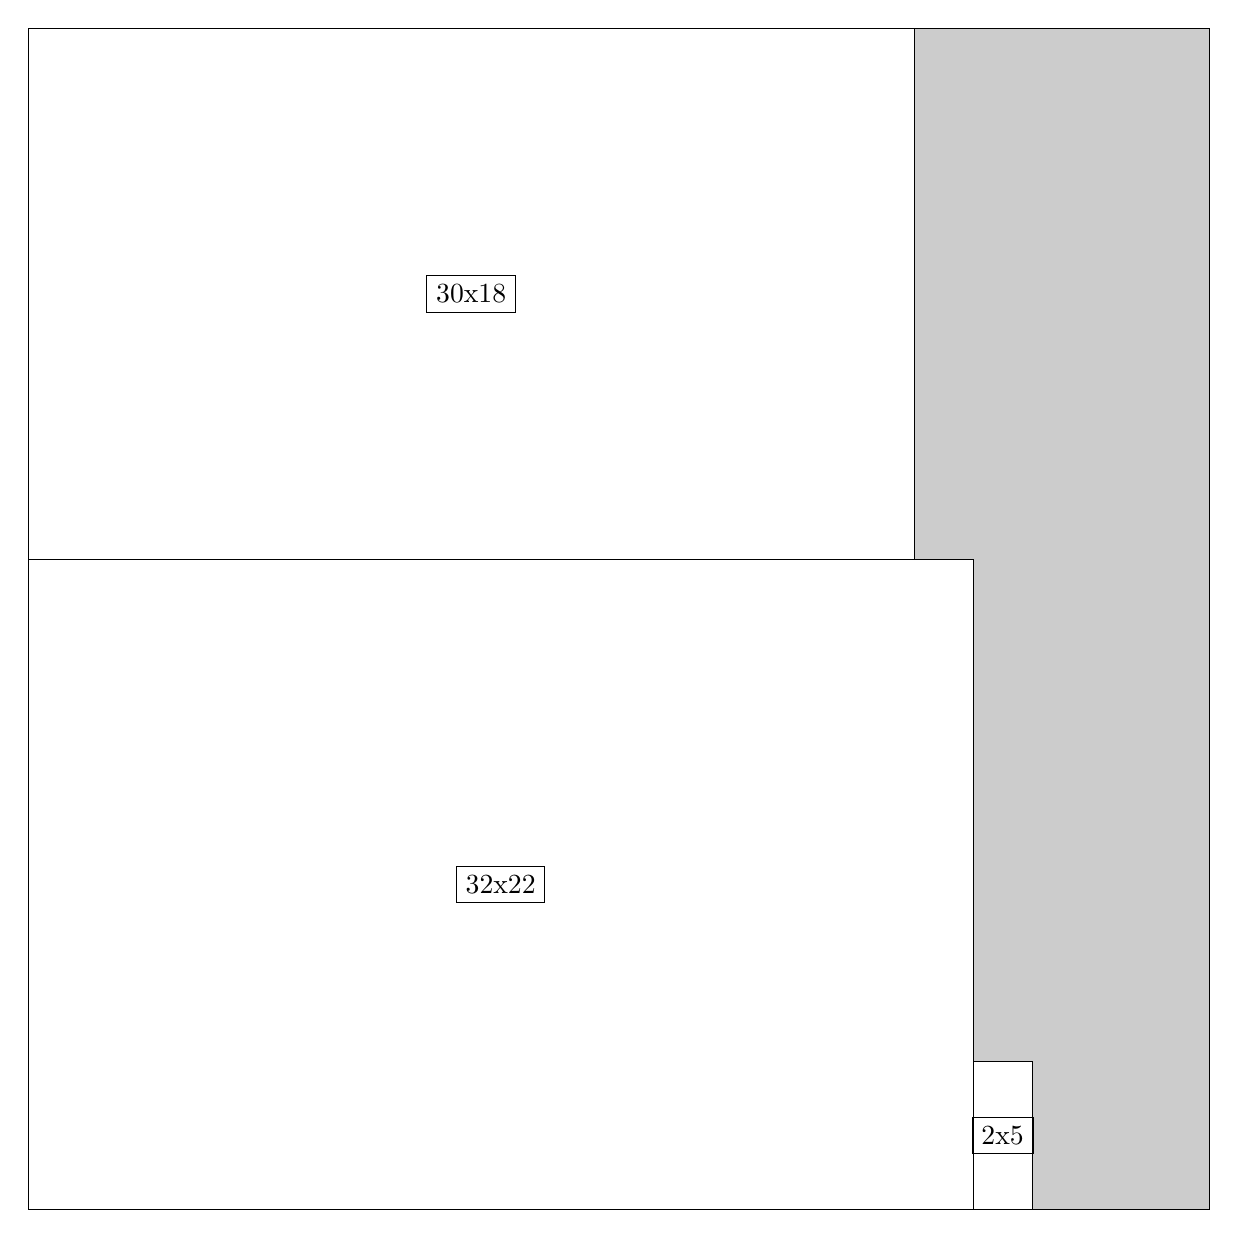
\begin{tikzpicture}[shorten >=1pt,scale=1.0,every node/.style={scale=1.0},->]
\tikzstyle{vertex}=[circle,fill=black!25,minimum size=14pt,inner sep=0pt]
\filldraw[fill=gray!40!white, draw=black] (0,0) rectangle (15.0,15.0);
\foreach \name/\x/\y/\w/\h in {30x18/0.0/8.25/11.25/6.75,32x22/0.0/0.0/12.0/8.25,2x5/12.0/0.0/0.75/1.875}
\filldraw[fill=white!40!white, draw=black] (\x,\y) rectangle node[draw] (\name) {\name} ++(\w,\h);
\end{tikzpicture}


w =30 , h =18 , x =0 , y =22 , v =540
\par
w =32 , h =22 , x =0 , y =0 , v =704
\par
w =2 , h =5 , x =32 , y =0 , v =10
\par
\newpage


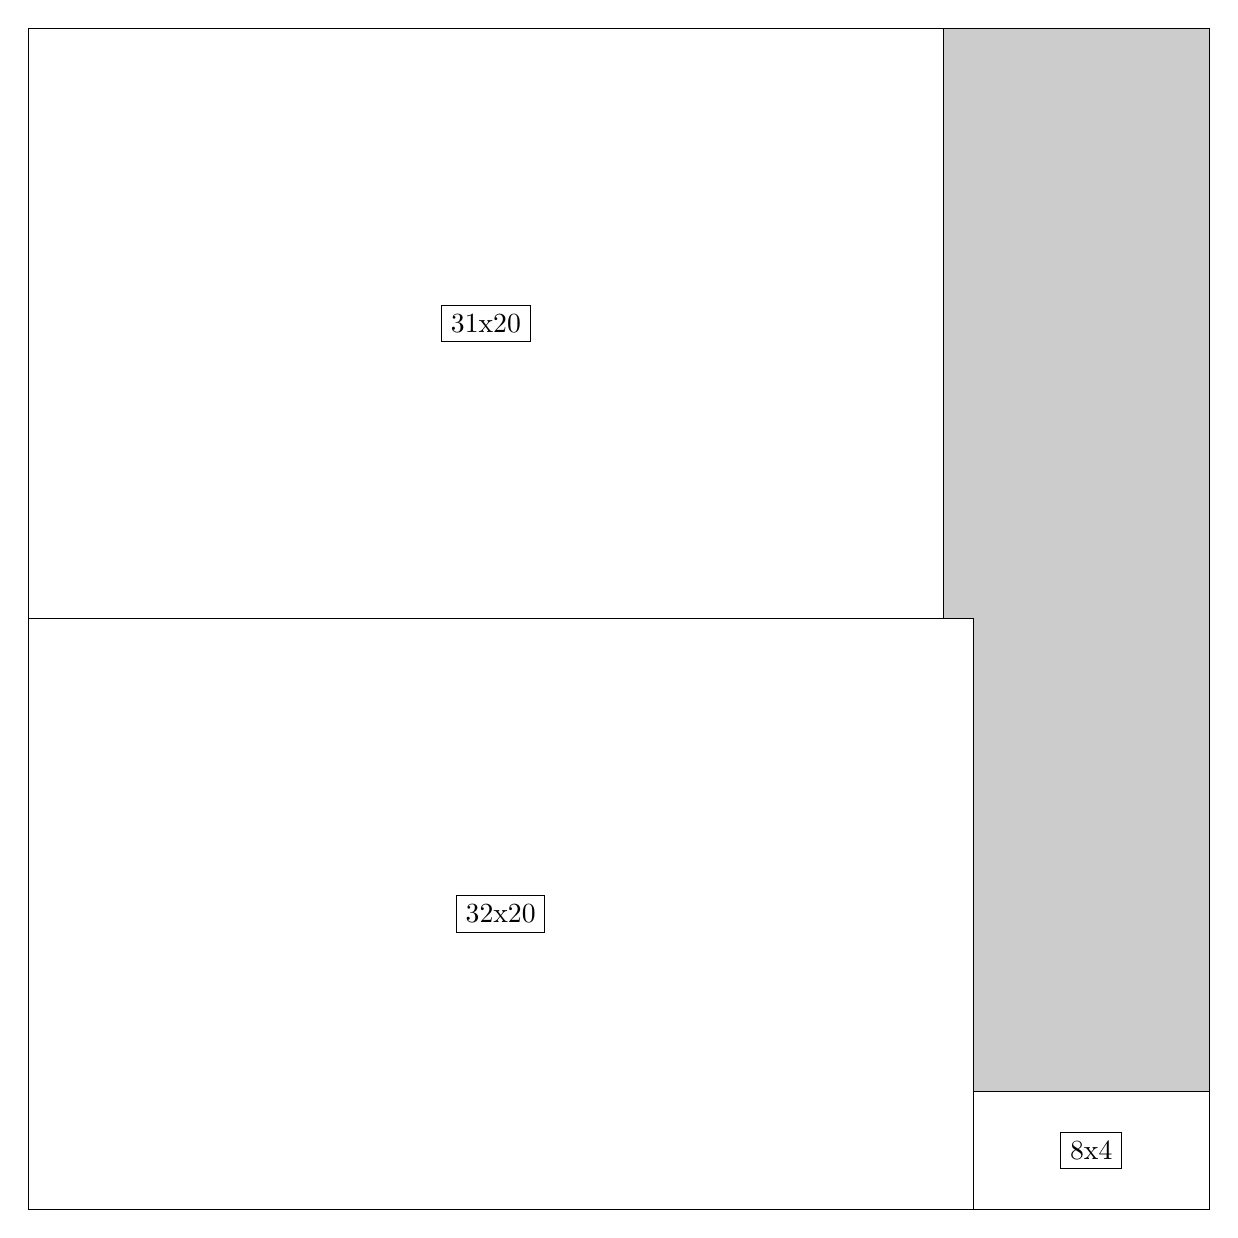
\begin{tikzpicture}[shorten >=1pt,scale=1.0,every node/.style={scale=1.0},->]
\tikzstyle{vertex}=[circle,fill=black!25,minimum size=14pt,inner sep=0pt]
\filldraw[fill=gray!40!white, draw=black] (0,0) rectangle (15.0,15.0);
\foreach \name/\x/\y/\w/\h in {32x20/0.0/0.0/12.0/7.5,31x20/0.0/7.5/11.625/7.5,8x4/12.0/0.0/3.0/1.5}
\filldraw[fill=white!40!white, draw=black] (\x,\y) rectangle node[draw] (\name) {\name} ++(\w,\h);
\end{tikzpicture}


w =32 , h =20 , x =0 , y =0 , v =640
\par
w =31 , h =20 , x =0 , y =20 , v =620
\par
w =8 , h =4 , x =32 , y =0 , v =32
\par
\newpage


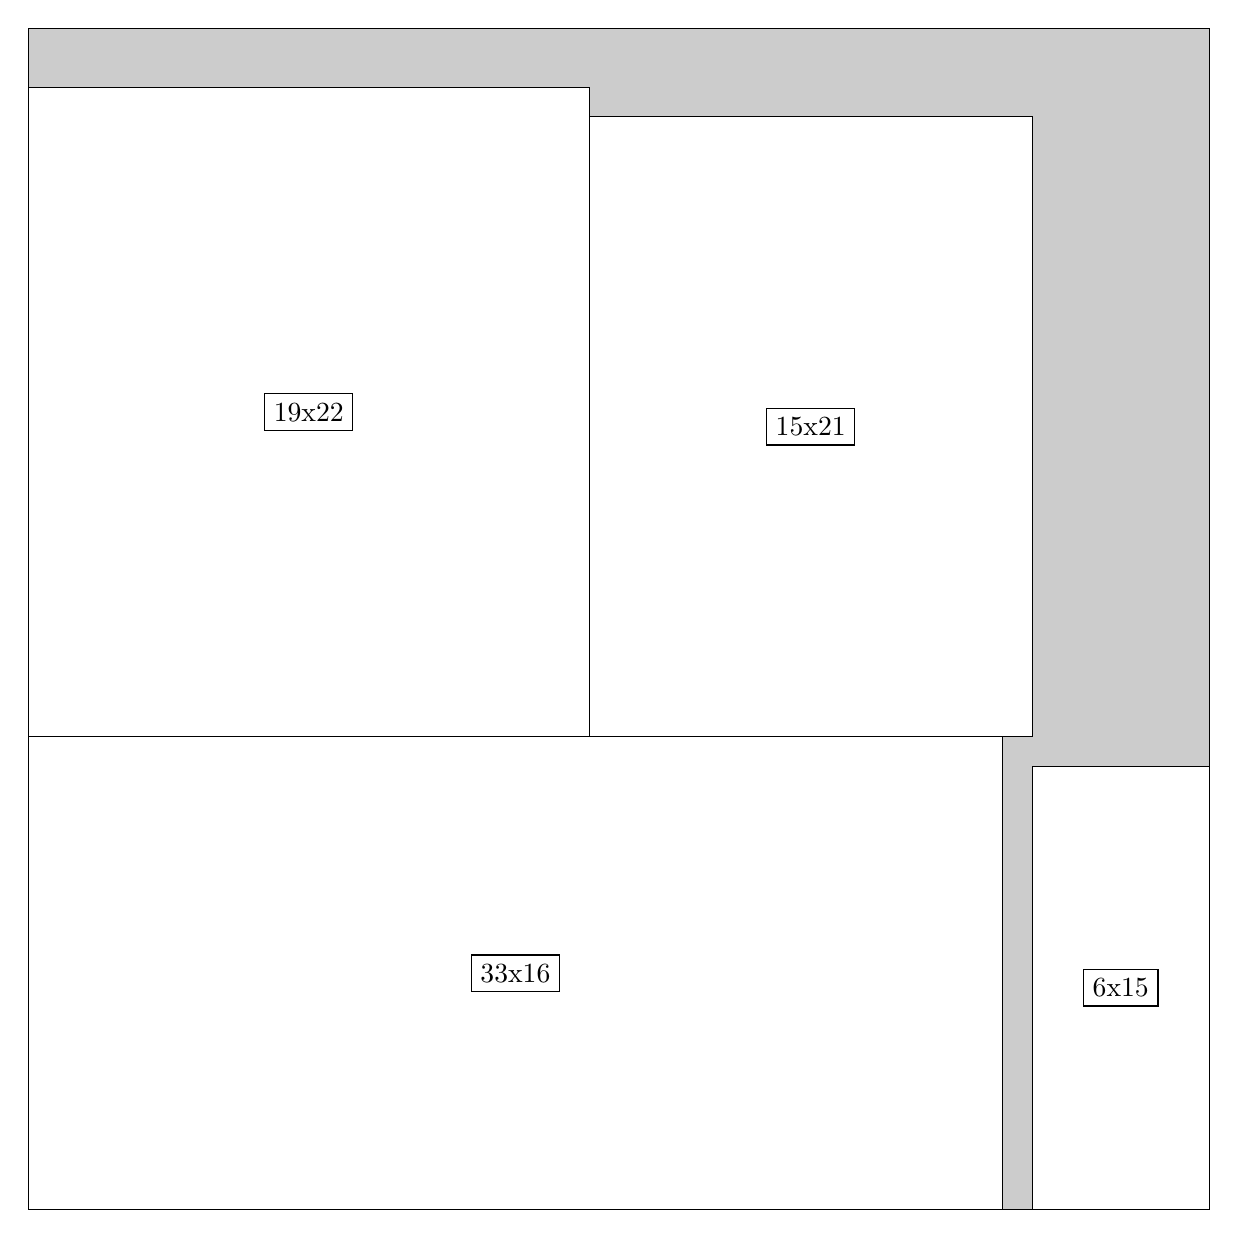
\begin{tikzpicture}[shorten >=1pt,scale=1.0,every node/.style={scale=1.0},->]
\tikzstyle{vertex}=[circle,fill=black!25,minimum size=14pt,inner sep=0pt]
\filldraw[fill=gray!40!white, draw=black] (0,0) rectangle (15.0,15.0);
\foreach \name/\x/\y/\w/\h in {33x16/0.0/0.0/12.375/6.0,19x22/0.0/6.0/7.125/8.25,15x21/7.125/6.0/5.625/7.875,6x15/12.75/0.0/2.25/5.625}
\filldraw[fill=white!40!white, draw=black] (\x,\y) rectangle node[draw] (\name) {\name} ++(\w,\h);
\end{tikzpicture}


w =33 , h =16 , x =0 , y =0 , v =528
\par
w =19 , h =22 , x =0 , y =16 , v =418
\par
w =15 , h =21 , x =19 , y =16 , v =315
\par
w =6 , h =15 , x =34 , y =0 , v =90
\par
\newpage


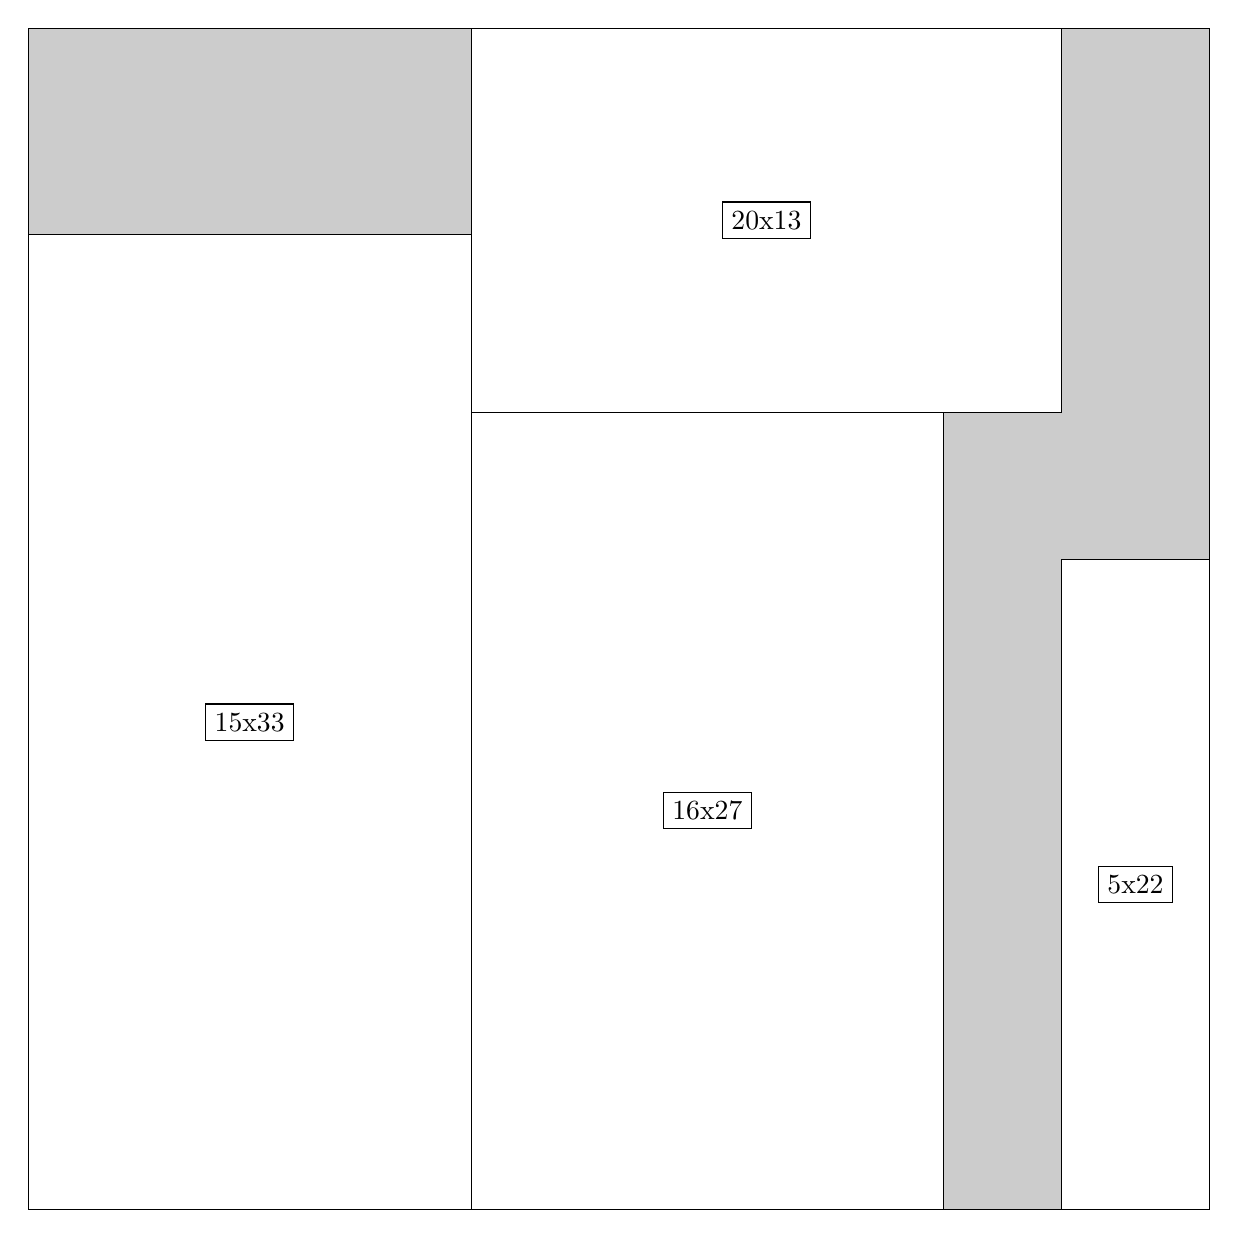
\begin{tikzpicture}[shorten >=1pt,scale=1.0,every node/.style={scale=1.0},->]
\tikzstyle{vertex}=[circle,fill=black!25,minimum size=14pt,inner sep=0pt]
\filldraw[fill=gray!40!white, draw=black] (0,0) rectangle (15.0,15.0);
\foreach \name/\x/\y/\w/\h in {15x33/0.0/0.0/5.625/12.375,16x27/5.625/0.0/6.0/10.125,20x13/5.625/10.125/7.5/4.875,5x22/13.125/0.0/1.875/8.25}
\filldraw[fill=white!40!white, draw=black] (\x,\y) rectangle node[draw] (\name) {\name} ++(\w,\h);
\end{tikzpicture}


w =15 , h =33 , x =0 , y =0 , v =495
\par
w =16 , h =27 , x =15 , y =0 , v =432
\par
w =20 , h =13 , x =15 , y =27 , v =260
\par
w =5 , h =22 , x =35 , y =0 , v =110
\par
\newpage


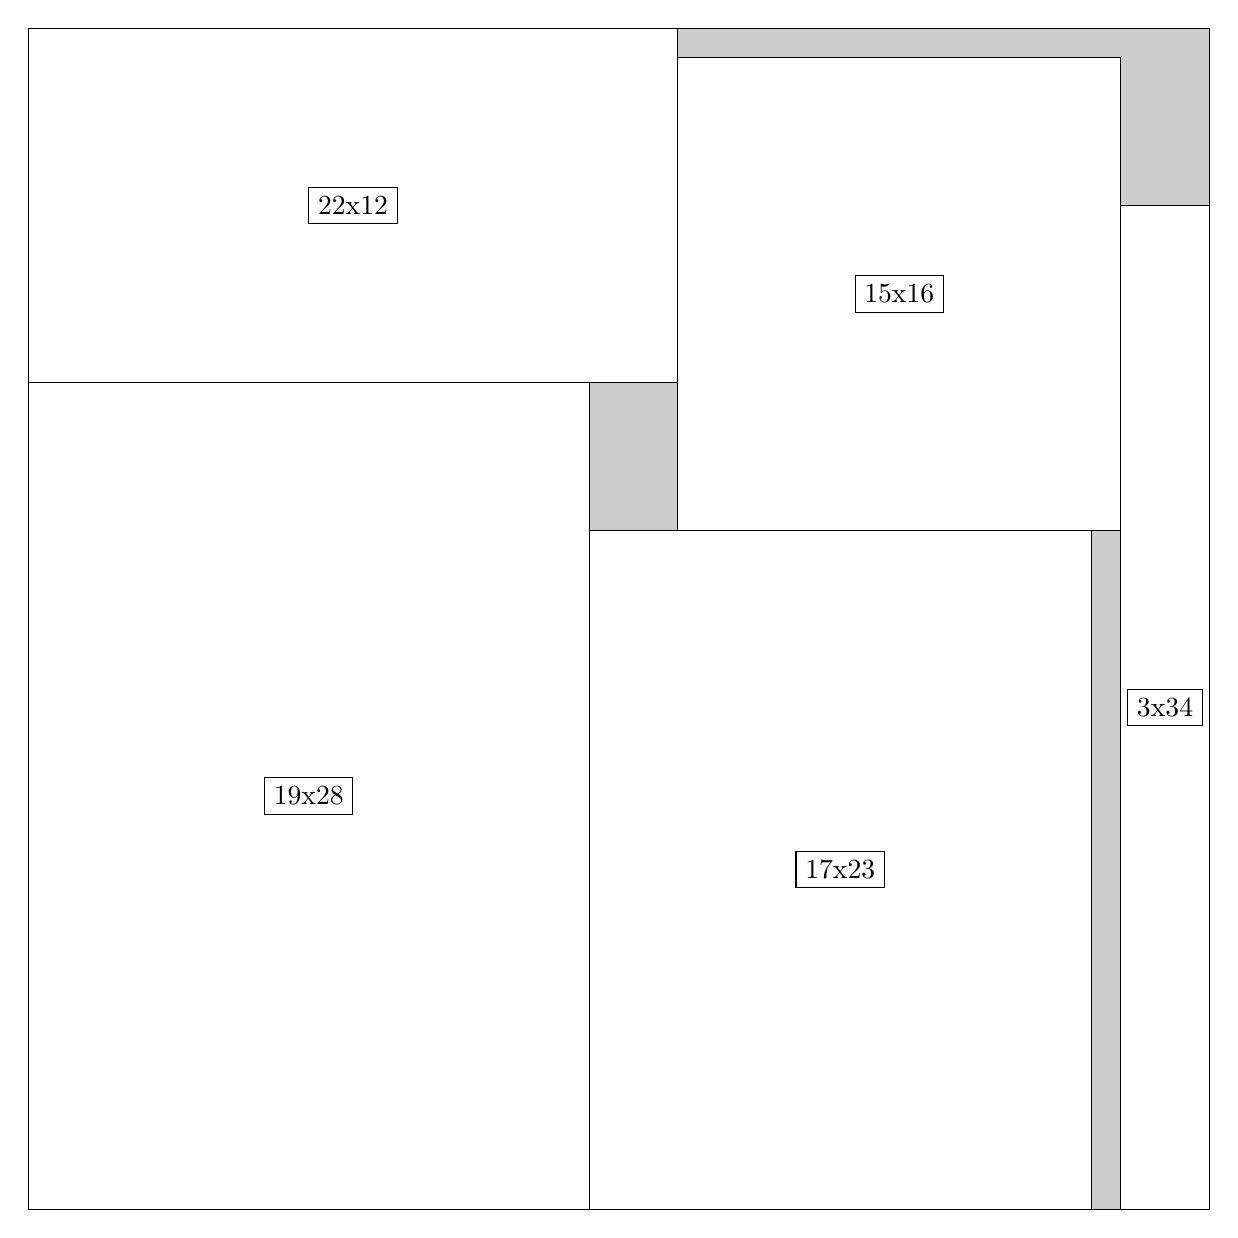
\begin{tikzpicture}[shorten >=1pt,scale=1.0,every node/.style={scale=1.0},->]
\tikzstyle{vertex}=[circle,fill=black!25,minimum size=14pt,inner sep=0pt]
\filldraw[fill=gray!40!white, draw=black] (0,0) rectangle (15.0,15.0);
\foreach \name/\x/\y/\w/\h in {19x28/0.0/0.0/7.125/10.5,17x23/7.125/0.0/6.375/8.625,22x12/0.0/10.5/8.25/4.5,15x16/8.25/8.625/5.625/6.0,3x34/13.875/0.0/1.125/12.75}
\filldraw[fill=white!40!white, draw=black] (\x,\y) rectangle node[draw] (\name) {\name} ++(\w,\h);
\end{tikzpicture}


w =19 , h =28 , x =0 , y =0 , v =532
\par
w =17 , h =23 , x =19 , y =0 , v =391
\par
w =22 , h =12 , x =0 , y =28 , v =264
\par
w =15 , h =16 , x =22 , y =23 , v =240
\par
w =3 , h =34 , x =37 , y =0 , v =102
\par
\newpage


\end{document}